% -------------------------
%	Author: ToanHac
%	Created: 22.10.2026
% -------------------------
\documentclass[a4paper]{article}
\usepackage{amssymb,epsfig,latexsym,multicol,array,hhline,fancyhdr}
\usepackage[utf8]{vntex}
\usepackage{amsmath}
\usepackage{amssymb}
\usepackage{lastpage}
\usepackage{indentfirst}
\usepackage[lined,boxed,commentsnumbered]{algorithm2e}
\usepackage{enumerate}
\usepackage{color}
\usepackage{graphicx}							% Standard graphics package
\usepackage{array}
\usepackage{tabularx, caption}
\usepackage{multirow}
\usepackage{multicol}
\usepackage{rotating}
\usepackage{graphics}
\usepackage[a4paper, top=2.5cm, bottom=2.5cm, left=2.5cm, right=2.5cm]{geometry}
\usepackage{setspace}
\usepackage{epsfig}
\usepackage{tikz}
\usetikzlibrary{arrows,backgrounds,shapes,positioning,calc}
\usepackage{hyperref}
\hypersetup{urlcolor=blue,linkcolor=black,citecolor=black,colorlinks=true} 
\usepackage{subcaption}
\usepackage{pgfplots}
\pgfplotsset{compat=1.15}
\usepackage{mathrsfs}
\usepackage{booktabs}
\usepackage{float}

\usepackage{listings}
% -- Defining colors:
\definecolor{codegray}{rgb}{0.5,0.5,0.5}
\definecolor{codegreen}{rgb}{0,0.6,0}
\definecolor{codepurple}{rgb}{0.58,0,0.82}
\definecolor{bg}{HTML}{F6F8FA} % Background color
\definecolor{keyword}{HTML}{D73A49} % Keyword color
\definecolor{identifier}{HTML}{005CC5} % Identifier color
\definecolor{builtin}{HTML}{6F42C1} % Builtin color

\definecolor{note}{HTML}{0000FF} % Blue color for word
% Defining a custom style for python code:
\lstdefinestyle{python}{
    language=Python,
    backgroundcolor=\color{bg},
    commentstyle=\color{codegreen},
    keywordstyle=\color{keyword}\bfseries,
    stringstyle=\color{codepurple},
    numberstyle=\tiny\color{codegray},
    identifierstyle=\color{identifier},
    basicstyle=\ttfamily\footnotesize,
    breaklines=true,
    keepspaces=true,                 
    numbers=left,       
    numbersep=5pt,
    frame=single,
    showspaces=false,
    tabsize=2,
    showstringspaces=false,
    morekeywords={self, True, False, None},
    framexleftmargin=3.5mm,
    linewidth=0.98\linewidth,
    xleftmargin=12pt,
    aboveskip=8pt,
    belowskip=8pt,
    rulecolor=\color{codegray},
}

\DeclareMathOperator*{\argmax}{argmax}
\DeclareMathOperator*{\argmin}{argmin}

\AtBeginDocument{\renewcommand*\contentsname{Mục lục}}
\AtBeginDocument{\renewcommand*\refname{Tài liệu tham khảo}}
\AtBeginDocument{\renewcommand*\figurename{Hình}}
\AtBeginDocument{\renewcommand*\tablename{Bảng}}

\setlength{\headheight}{30pt}
\pagestyle{fancy}
\fancyhead{} % clear all header fields
\fancyhead[L]{
 \begin{tabular}{rl}
    \begin{picture}(25,15)(0,0)
    \put(0,-8){
\includegraphics[width=8mm, height=8mm]{Images/hcmut.png}}
   \end{picture}&
	\begin{tabular}{l}
		\textbf{\bf \ttfamily Trường Đại học Bách khoa, Tp. Hồ Chí Minh}\\
		\textbf{\bf \ttfamily Khoa Khoa học và Kỹ thuật máy tính}
	\end{tabular} 	
 \end{tabular}
}
\fancyhead[R]{
	\begin{tabular}{l}
		\tiny \bf \\
		\tiny \bf 
	\end{tabular}  }
\fancyfoot{} % clear all footer fields
\fancyfoot[L]{\scriptsize \ttfamily Nhập môn trí tuệ nhân tạo - Học kỳ 261}
\fancyfoot[R]{\scriptsize \ttfamily Trang {\thepage}/\pageref{LastPage}}
\renewcommand{\headrulewidth}{0.3pt}
\renewcommand{\footrulewidth}{0.3pt}


%%%
\setcounter{secnumdepth}{4}
\setcounter{tocdepth}{3}
\makeatletter
\newcounter {subsubsubsection}[subsubsection]
\renewcommand\thesubsubsubsection{\thesubsubsection .\@alph\c@subsubsubsection}
\newcommand\subsubsubsection{\@startsection{subsubsubsection}{4}{\z@}%
                                     {-3.25ex\@plus -1ex \@minus -.2ex}%
                                     {1.5ex \@plus .2ex}%
                                     {\normalfont\normalsize\bfseries}}
\newcommand*\l@subsubsubsection{\@dottedtocline{3}{10.0em}{4.1em}}
\newcommand*{\subsubsubsectionmark}[1]{}
\makeatother

% Cho phép ngắt dòng linh hoạt với các từ inline code dài
\sloppy

% Macro hỗ trợ vẽ mảnh ống nước trực quan bằng TikZ
\newcommand{\drawpipe}[6][0.58]{
    % #1: scale (default 0.58), #2: North, #3: East, #4: South, #5: West, #6: Color
    \begin{tikzpicture}[scale=#1]
        \fill[gray!10, rounded corners=2pt] (-1,-1) rectangle (1,1);
        \draw[gray!50, thin, rounded corners=2pt] (-1,-1) rectangle (1,1);
        \ifnum#2=1 \draw[#6, line width=3.5pt, line cap=butt] (0,0) -- (0,1); \fi
        \ifnum#3=1 \draw[#6, line width=3.5pt, line cap=butt] (0,0) -- (1,0); \fi
        \ifnum#4=1 \draw[#6, line width=3.5pt, line cap=butt] (0,0) -- (0,-1); \fi
        \ifnum#5=1 \draw[#6, line width=3.5pt, line cap=butt] (0,0) -- (-1,0); \fi
        \fill[#6] (0,0) circle (0.28);
    \end{tikzpicture}
}

\begin{document}

\begin{titlepage}
\begin{tikzpicture}[remember picture,overlay,inner sep=0,outer sep=0]
	\draw[blue!70!black,line width=4pt] ([xshift=-1.5cm,yshift=-1.8cm]current page.north east) coordinate (A)--([xshift=1.5cm,yshift=-1.8cm]current page.north west) coordinate(B)--([xshift=1.5cm,yshift=1.8cm]current page.south west) coordinate (C)--([xshift=-1.5cm,yshift=1.8cm]current page.south east) coordinate(D)--cycle;
\end{tikzpicture}
\begin{center}
\textbf{\large ĐẠI HỌC QUỐC GIA TP. HỒ CHÍ MINH} \\
\textbf{\large TRƯỜNG ĐẠI HỌC BÁCH KHOA} \\
\textbf{\large KHOA KHOA HỌC VÀ KỸ THUẬT MÁY TÍNH}
\end{center}


\vspace{0.8cm}

\begin{figure}[h!]
\begin{center}

\includegraphics[width=3cm]{Images/hcmut.png}
\end{center}
\end{figure}

\vspace{0.6cm}


\begin{center}
\begin{tabular}{c}
\textbf{\Large NHẬP MÔN TRÍ TUỆ NHÂN TẠO} \\[0.3cm]
\hline
\\[-0.1cm]
\textbf{\Large BÁO CÁO BÀI TẬP LỚN 1} \\[0.3cm]
\textbf{\huge GIẢI BÀI TOÁN LOGIC PUZZLE PIPES} \\[0.3cm]
\textbf{\large BẰNG GIẢI THUẬT TÌM KIẾM MÙ VÀ HEURISTIC} \\[0.3cm]
\hline
\end{tabular}
\end{center}

\vspace{0.8cm}

	\begin{table}[h]
    	\centering
    	\begin{tabular}{rlcl}
    		\textbf{GVHD:} & TS. Vương Bá Thịnh & & \\
    		\textbf{SV thực hiện:} & Hoa Toàn Hạc & -- & 2210917 \\
    		& ...... & -- & ..... \\
    	\end{tabular}
    \end{table}

\vspace{5cm}
\begin{center}
{\footnotesize \textbf{TP. HỒ CHÍ MINH, THÁNG 10 NĂM 2026}}
\end{center}
\end{titlepage}


%\thispagestyle{empty}

\tableofcontents
\newpage

% =====================================================================
% LỜI MỞ ĐẦU
% =====================================================================
\section*{Lời mở đầu}
\addcontentsline{toc}{section}{Lời mở đầu}

Trong lĩnh vực Trí tuệ nhân tạo, các giải thuật tìm kiếm trong không gian trạng thái đóng vai trò nền tảng cho việc giải quyết các bài toán lập kế hoạch, tối ưu hóa tổ hợp và trò chơi logic. Thông qua việc biểu diễn một vấn đề thực tế thành các trạng thái, hành động chuyển tiếp và điều kiện đích, máy tính có thể tự động tìm kiếm và đưa ra lời giải hợp lệ mà không cần sự can thiệp trực tiếp của con người.

Trong khuôn khổ Bài tập lớn 1 môn Nhập môn Trí tuệ nhân tạo (HK1 năm học 2026--2027), nhóm lựa chọn nghiên cứu và giải quyết bài toán Puzzle Pipes trên hệ thống \href{https://www.puzzle-pipes.com/}{\texttt{puzzle-pipes.com}}. Đây là bài toán thỏa mãn ràng buộc kết hợp với tính chất liên thông đồ thị toàn cục: mỗi thao tác xoay ống tại một ô không chỉ ảnh hưởng đến 4 ô láng giềng trực tiếp mà còn quyết định việc toàn bộ mạng lưới có bị phân mảnh hay tạo chu trình khép kín hay không.

Để giải quyết bài toán này theo đúng yêu cầu của đề bài, nhóm đã xây dựng một hệ thống hoàn chỉnh bằng ngôn ngữ Python 3, bao gồm các nội dung chính:
\begin{enumerate}
    \item Mô hình hóa toán học bằng Bitmask 4-bit: Tối ưu hóa việc lưu trữ hướng của từng mảnh ống và biến phép xoay hình học $90^\circ$ thành phép dịch bit tròn với độ phức tạp thời gian $O(1)$.
    \item Hiện thực hai trường phái giải thuật tìm kiếm:
    \begin{itemize}
        \item Tìm kiếm mù (Blind Search): Giải thuật tìm kiếm theo chiều sâu Depth-First Search (DFS) kết hợp quay lui (Backtracking) và kỹ thuật cắt tỉa nhánh sớm (Forward Pruning).
        \item Tìm kiếm có thông tin (Heuristic Search): Giải thuật $A^*$ Search sử dụng cấu trúc hàng đợi ưu tiên (Min-Heap) với hàm đánh giá $f(n) = g(n) + h(n)$ dựa trên số cổng xung đột cục bộ, thỏa mãn tính chất chấp nhận được (Admissible).
    \end{itemize}
    \item Trình sinh bàn cờ ngẫu nhiên luôn có nghiệm dựa trên thuật toán cây khung ngẫu nhiên (Randomized Spanning Tree), tạo bộ dữ liệu kiểm thử từ kích thước $3 \times 3$ đến $8 \times 8$.
    \item Giao diện trực quan hóa tương tác (Web Visualizer Step-by-Step) xây dựng trên nền tảng Flask và HTML5/CSS3/SVG, cho phép theo dõi trực quan từng bước xoay ống, quay lui, điều chỉnh tốc độ phát và đối chiếu thông số hiệu năng.
\end{enumerate}

Báo cáo dưới đây trình bày chi tiết quá trình tìm hiểu, mô hình hóa, thiết kế giải thuật, kết quả đo đạc thời gian thực thi -- bộ nhớ tiêu thụ cùng những phân tích đánh giá của nhóm.

\newpage

% =====================================================================
% PHẦN 1: GIỚI THIỆU VÀ MÔ HÌNH HÓA BÀI TOÁN
% =====================================================================
\section{Giới thiệu và Mô hình hóa bài toán}

\subsection{Mô tả trò chơi Logic Puzzle Pipes}
Puzzle Pipes (còn được gọi là Net hoặc FreeNet) là trò chơi giải đố logic trên trang web \href{https://www.puzzle-pipes.com/}{\texttt{puzzle-pipes.com}}. Trò chơi diễn ra trên một bảng lưới hai chiều kích thước $R \times C$ (thường là lưới vuông $N \times N$). Tại mỗi ô $(r, c)$ của lưới chứa một mảnh đường ống dẫn nước thuộc một trong năm hình dạng cơ bản:
\begin{itemize}
    \item Ống cụt (End pipe): Chỉ có $1$ cổng kết nối, đóng vai trò là điểm đầu hoặc điểm cuối của nhánh ống.
    \item Ống thẳng (Straight pipe): Có $2$ cổng kết nối nằm đối diện nhau ($180^\circ$).
    \item Ống góc vuông (Turn pipe): Có $2$ cổng kết nối vuông góc với nhau ($90^\circ$).
    \item Ống chữ T (Tee junction): Có $3$ cổng kết nối tỏa ra 3 hướng.
    \item Ống chữ thập (Cross pipe): Có $4$ cổng kết nối tỏa ra cả 4 hướng.
\end{itemize}

Ở trạng thái khởi đầu, tất cả các mảnh ống trên bàn cờ bị xoay ngẫu nhiên làm đứt gãy mạch nước. Người chơi hoặc tác tử AI chỉ được phép xoay tại chỗ từng mảnh ống theo các góc $90^\circ, 180^\circ, 270^\circ$ mà không được hoán đổi vị trí giữa các ô. Trò chơi kết thúc thành công khi toàn bộ các mảnh ống trên bàn cờ thỏa mãn đồng thời 3 điều kiện:
\begin{enumerate}
    \item Không hở biên: Không có bất kỳ cổng kết nối nào hướng ra ngoài ranh giới bức tường bao quanh bàn cờ.
    \item Khớp nối hoàn toàn: Mọi cổng mở của một ô phải nối khớp trực tiếp với một cổng mở hướng ngược lại của ô láng giềng liền kề.
    \item Liên thông toàn cục: Tất cả các ô có ống nước trên bàn cờ phải kết nối với nhau tạo thành duy nhất một mạng lưới liên thông (cây khung dẫn nước từ nguồn tới mọi điểm), không có bất kỳ cụm ống nào bị cô lập tách rời.
\end{enumerate}

\subsection{Biểu diễn Toán học bằng Hệ thống Bitmask 4-bit}
Để tối ưu tốc độ kiểm tra ràng buộc trong quá trình tìm kiếm, nhóm biểu diễn mỗi mảnh ống bằng một số nguyên 4-bit (Bitmask) trong đoạn $[0, 15]$ tương ứng với 4 hướng địa lý: Bắc (NORTH), Đông (EAST), Nam (SOUTH) và Tây (WEST).

Quy ước trọng số bit như sau:
\begin{equation}
    \text{Mask} = (b_3 b_2 b_1 b_0)_2 = b_3 \cdot 2^3 + b_2 \cdot 2^2 + b_1 \cdot 2^1 + b_0 \cdot 2^0
\end{equation}
Trong đó:
\begin{itemize}
    \item Bit $0$ ($\text{NORTH} = 1 = 0001_2$): Cổng nối lên phía trên $\Delta = (-1, 0)$, hướng đối diện là $\text{SOUTH}$ ($4$).
    \item Bit $1$ ($\text{EAST} = 2 = 0010_2$): Cổng nối sang bên phải $\Delta = (0, +1)$, hướng đối diện là $\text{WEST}$ ($8$).
    \item Bit $2$ ($\text{SOUTH} = 4 = 0100_2$): Cổng nối xuống phía dưới $\Delta = (+1, 0)$, hướng đối diện là $\text{NORTH}$ ($1$).
    \item Bit $3$ ($\text{WEST} = 8 = 1000_2$): Cổng nối sang bên trái $\Delta = (0, -1)$, hướng đối diện là $\text{EAST}$ ($2$).
\end{itemize}

\begin{figure}[H]
\centering
\setlength{\tabcolsep}{4pt}
\small
\begin{tabular}{cccccc}
\drawpipe[0.52]{1}{0}{0}{0}{blue!70!black} &
\drawpipe[0.52]{0}{1}{0}{1}{blue!70!black} &
\drawpipe[0.52]{1}{1}{0}{0}{blue!70!black} &
\drawpipe[0.52]{0}{1}{1}{0}{blue!70!black} &
\drawpipe[0.52]{1}{1}{0}{1}{blue!70!black} &
\drawpipe[0.52]{1}{1}{1}{1}{blue!70!black} \\
Mask = 1 & Mask = 10 & Mask = 3 & Mask = 6 & Mask = 11 & Mask = 15 \\
\texttt{(0001\textsubscript{2})} & \texttt{(1010\textsubscript{2})} & \texttt{(0011\textsubscript{2})} & \texttt{(0110\textsubscript{2})} & \texttt{(1011\textsubscript{2})} & \texttt{(1111\textsubscript{2})} \\
Ống cụt (N) & Ống thẳng (E-W) & Ống góc (N-E) & Ống góc (E-S) & Chữ T (N-E-W) & Chữ thập \\
\end{tabular}
\caption{Minh họa trực quan các loại mảnh ống và mã hóa Bitmask 4-bit tương ứng.}
\label{fig:bitmask_pipes}
\end{figure}

Khi xoay một mảnh ống $90^\circ$ theo chiều kim đồng hồ ($\text{NORTH} \to \text{EAST} \to \text{SOUTH} \to \text{WEST} \to \text{NORTH}$), các bit ở vị trí $0, 1, 2$ dịch sang trái 1 bậc, còn bit thứ $3$ ($\text{WEST}$) vòng về vị trí bit $0$ ($\text{NORTH}$). Do đó, phép xoay $90^\circ$ được tính trực tiếp bằng phép dịch bit tròn:
\begin{equation}
    \text{RotateCW}(\text{mask}) = \big((\text{mask} \ll 1) \ \& \ 15\big) \ \mid \ (\text{mask} \gg 3)
\end{equation}

Nhờ tính đối xứng hình học, số lượng hướng quay phân biệt của mỗi ô được rút gọn:
\begin{itemize}
    \item Ống cụt, ống góc, ống chữ T: Có $4$ trạng thái quay phân biệt.
    \item Ống thẳng ($\text{mask} \in \{5, 10\}$): Chỉ có $2$ trạng thái phân biệt (dọc $5$ và ngang $10$), giúp giảm một nửa hệ số phân nhánh tại các ô này.
    \item Ống chữ thập ($\text{mask} = 15$) hoặc ô trống ($0$): Chỉ có $1$ trạng thái duy nhất.
\end{itemize}

\subsection{Mô hình hóa Bài toán Tìm kiếm (State Space Formulation)}
Bài toán Puzzle Pipes trên lưới kích thước $R \times C$ được định nghĩa hình thức qua bộ 5 thành phần $\mathcal{P} = \langle \mathcal{S}, s_0, \mathcal{A}, \mathcal{T}, \mathcal{G} \rangle$:

\begin{enumerate}
    \item Không gian trạng thái ($\mathcal{S}$):
    Một trạng thái $s \in \mathcal{S}$ được biểu diễn bởi cặp $(k, M)$, trong đó:
    \begin{itemize}
        \item $k \in \{0, 1, \dots, R \times C\}$ là số lượng ô đã được cố định hướng theo thứ tự dòng quét từ trái sang phải, từ trên xuống dưới (chỉ số ô $i = r \times C + c$).
        \item $M \in \{0, \dots, 15\}^{R \times C}$ là ma trận cấu hình bitmask hiện tại của các mảnh ống trên bàn cờ.
    \end{itemize}
    Nếu không áp dụng cắt tỉa, kích thước không gian trạng thái lý thuyết có thể lên tới $|\mathcal{S}| = \prod_{r,c} |\text{Rotations}(M_{r,c})| \le 4^{R \times C}$ (với lưới $8 \times 8$, $4^{64} \approx 3.4 \times 10^{38}$ trạng thái).

    \item Trạng thái ban đầu ($s_0$):
    Trạng thái $s_0 = (0, M_{\text{init}})$, trong đó chưa có ô nào được cố định hướng ($k = 0$) và $M_{\text{init}}$ là ma trận bitmask đọc từ tệp dữ liệu đầu vào hoặc từ bộ sinh ngẫu nhiên.

    \item Tập hành động hợp lệ ($\mathcal{A}(s)$) và Ràng buộc khớp cục bộ:
    Tại trạng thái $s = (k, M)$ tương ứng với ô hiện tại $(r, c)$ (với $r = \lfloor k / C \rfloor, c = k \bmod C$), tập hành động $\mathcal{A}(s)$ là việc chọn một cấu hình xoay $m' \in \text{UniqueRotations}(M_{r,c})$ thỏa mãn điều kiện tương thích cục bộ:
    \begin{itemize}
        \item Ràng buộc biên: Với mọi hướng $d \in \{\text{N, E, S, W}\}$, nếu $(m' \ \& \ d) \neq 0$ thì tọa độ láng giềng $(r + \Delta r_d, c + \Delta c_d)$ phải nằm trong phạm vi bàn cờ $0 \le nr < R, 0 \le nc < C$.
        \item Ràng buộc khớp láng giềng đã gán: Với mọi ô láng giềng $(nr, nc)$ đã được cố định hướng trước đó (ô phía trên $(r-1, c)$ và ô bên trái $(r, c-1)$), trạng thái cổng nối giữa hai ô phải khớp nhau:
        \begin{equation}
            \big((m' \ \& \ d) \neq 0\big) \iff \big((M_{nr,nc} \ \& \ \text{OPPOSITE}[d]) \neq 0\big)
        \end{equation}
    \end{itemize}

    \item Hàm chuyển trạng thái ($\mathcal{T}(s, a)$):
    Khi thực hiện hành động gán hướng $m'$ cho ô thứ $k$ tại tọa độ $(r, c)$, trạng thái chuyển từ $s = (k, M)$ sang trạng thái kế tiếp $s' = (k + 1, M')$, trong đó $M'_{r,c} = m'$ và các ô khác giữ nguyên giá trị.

    \item Kiểm tra trạng thái đích ($\mathcal{G}(s)$):
    Một trạng thái hoàn chỉnh $s = (R \times C, M)$ là trạng thái đích khi và chỉ khi:
    \begin{itemize}
        \item Điều kiện 1 (Khớp cục bộ toàn bàn cờ): Mọi ô $(r, c)$ không có cổng chỉ ra ngoài tường và khớp với cả 4 ô láng giềng xung quanh.
        \item Điều kiện 2 (Liên thông toàn cục bằng BFS): Khởi chạy thuật toán duyệt theo chiều rộng (BFS) từ một ô có ống nước đầu tiên $(r_{\text{start}}, c_{\text{start}})$, đi theo các cổng kết nối mở. Số lượng ô thăm được $|\text{visited}|$ phải bằng đúng tổng số ô chứa ống nước trên bàn cờ. Điều kiện này loại bỏ các nghiệm giả bị tách thành nhiều vòng khép kín độc lập.
    \end{itemize}
\end{enumerate}

\subsection{Đặc tả dữ liệu đầu vào và Thuật toán sinh bàn cờ có nghiệm}
Các tệp dữ liệu đầu vào trong thư mục \texttt{inputs/} được lưu dưới định dạng văn bản thuần (\texttt{.txt}). Dòng đầu tiên chứa hai số nguyên dương $R$ và $C$ biểu thị số hàng và số cột; $R$ dòng tiếp theo, mỗi dòng chứa $C$ số nguyên trong đoạn $[1, 15]$ biểu diễn mã bitmask ban đầu của từng mảnh ống.

Để đảm bảo mọi bộ dữ liệu kiểm thử từ $3 \times 3$ đến $8 \times 8$ đều chắc chắn có lời giải hợp lệ, nhóm xây dựng thuật toán sinh bàn cờ dựa trên Cây khung ngẫu nhiên (Randomized Spanning Tree via DFS):
\begin{enumerate}
    \item Khởi tạo lưới rỗng $R \times C$ với mọi ô có bitmask bằng $0$.
    \item Xuất phát từ ô $(0, 0)$, thực hiện duyệt DFS ngẫu nhiên (xáo trộn thứ tự 4 hướng ở mỗi bước). Mỗi khi đi từ ô $(r, c)$ sang ô chưa thăm $(nr, nc)$ theo hướng $d$, bật bit cổng $d$ tại ô $(r, c)$ và bật bit cổng đối diện $\text{OPPOSITE}[d]$ tại ô $(nr, nc)$.
    \item Khi toàn bộ $R \times C$ ô đã được thăm, ta thu được một cây khung liên thông hoàn chỉnh không chu trình làm nghiệm gốc.
    \item Cuối cùng, xoay ngẫu nhiên mỗi ô từ $0$ đến $3$ lần để xáo trộn hướng, tạo ra bàn cờ đề bài.
\end{enumerate}

\newpage

% =====================================================================
% PHẦN 2: CẤU TRÚC MÃ NGUỒN VÀ HIỆN THỰC GIẢI THUẬT
% =====================================================================
\section{Cấu trúc mã nguồn và Hiện thực giải thuật}

\subsection{Kiến trúc tổng thể của hệ thống}
Hệ thống được thiết kế theo kiến trúc phân tầng, tách biệt giữa lõi giải thuật AI, bộ công cụ đo đạc thực nghiệm và giao diện trực quan hóa Web.

\begin{figure}[H]
\centering
\begin{tikzpicture}[
    node distance=1.1cm and 1.4cm,
    box/.style={rectangle, draw=blue!70!black, fill=blue!5, thick, minimum width=3.5cm, minimum height=0.95cm, align=center, rounded corners=4pt, font=\footnotesize\sffamily},
    core/.style={rectangle, draw=orange!80!black, fill=orange!10, thick, minimum width=3.6cm, minimum height=0.95cm, align=center, rounded corners=4pt, font=\footnotesize\sffamily},
    ui/.style={rectangle, draw=teal!80!black, fill=teal!10, thick, minimum width=3.5cm, minimum height=0.95cm, align=center, rounded corners=4pt, font=\footnotesize\sffamily},
    arrow/.style={->, >=stealth, thick, draw=gray!80!black}
]
    % Nodes
    \node[box] (const) {\texttt{pipe\_constants.py}\\(Bitmask 4-bit \& Rotate)};
    \node[box, right=of const] (board) {\texttt{board.py}\\(Model, Local Match, BFS)};
    \node[box, right=of board] (gen) {\texttt{generator.py}\\(Spanning Tree Map Gen)};

    \node[core, below=1.1cm of board] (base) {\texttt{solver\_base.py}\\(\texttt{perf\_counter} \& \texttt{tracemalloc})};
    \node[core, below left=1.1cm and 0.3cm of base] (dfs) {\texttt{blind\_search.py}\\(DFSSolver: Backtracking)};
    \node[core, below right=1.1cm and 0.3cm of base] (astar) {\texttt{heuristic\_search.py}\\(AStarSolver: Min-Heap)};

    \node[ui, below=1.2cm of dfs] (bench) {\texttt{benchmark.py} \& \texttt{plot}\\(CSV \& High-Res Charts)};
    \node[ui, below=1.2cm of astar] (flask) {\texttt{app.py} \& Web UI\\(Flask API + SVG Step-by-Step)};

    % Arrows
    \draw[arrow] (const) -- (board);
    \draw[arrow] (const) to[bend left=18] (gen);
    \draw[arrow] (board) -- (gen);
    \draw[arrow] (board) -- (base);
    \draw[arrow] (base) -- (dfs);
    \draw[arrow] (base) -- (astar);
    \draw[arrow] (dfs) -- (bench);
    \draw[arrow] (astar) -- (bench);
    \draw[arrow] (dfs) -- (flask);
    \draw[arrow] (astar) -- (flask);
\end{tikzpicture}
\caption{Sơ đồ kiến trúc các module trong dự án Puzzle Pipes AI.}
\label{fig:architecture}
\end{figure}

Vai trò cụ thể của từng tệp mã nguồn trong dự án:
\begin{itemize}
    \item \texttt{src/pipe\_constants.py}: Định nghĩa hằng số hướng 4-bit, vector dịch chuyển $\Delta r, \Delta c$, phép xoay bit và hàm sinh các hướng quay không trùng lặp.
    \item \texttt{src/board.py}: Lớp \texttt{Board} quản lý lưới 2 chiều, đọc/ghi file, kiểm tra ràng buộc biên, kiểm tra khớp nối cục bộ, đếm xung đột và kiểm tra đích toàn cục bằng BFS.
    \item \texttt{src/solver\_base.py}: Lớp cơ sở \texttt{SolverBase} chuẩn hóa giao diện giải thuật, bọc bộ đo thời gian thực thi (\texttt{time.perf\_counter}) và bộ đo đỉnh bộ nhớ RAM (\texttt{tracemalloc}), đồng thời lưu vết từng bước xoay ống phục vụ trình chiếu Step-by-Step.
    \item \texttt{src/blind\_search.py}: Hiện thực lớp \texttt{DFSSolver} kế thừa từ \texttt{SolverBase}.
    \item \texttt{src/heuristic\_search.py}: Hiện thực lớp \texttt{AStarSolver} kế thừa từ \texttt{SolverBase}.
    \item \texttt{src/benchmark.py} và \texttt{src/plot\_benchmark.py}: Tự động chạy thực nghiệm trên toàn bộ các tệp trong \texttt{inputs/}, xuất bảng tổng hợp ra file CSV và vẽ biểu đồ 300 DPI.
    \item \texttt{app.py}, \texttt{templates/index.html}, \texttt{static/js/app.js}: Máy chủ Flask và giao diện Web tương tác.
\end{itemize}

\subsection{Giải thuật 1: Tìm kiếm mù -- DFS Backtracking kết hợp Forward Pruning}
\subsubsection{Nguyên lý hoạt động}
Trong bài toán Puzzle Pipes, một nghiệm hợp lệ luôn đòi hỏi mọi ô từ $(0, 0)$ đến $(R-1, C-1)$ đều phải được định hướng. Thay vì sử dụng tìm kiếm theo chiều rộng (BrFS) vốn gây bùng nổ bộ nhớ theo cấp số nhân ngay ở những hàng đầu tiên, nhóm lựa chọn giải thuật Tìm kiếm theo chiều sâu (DFS) kết hợp Quay lui (Backtracking) và kỹ thuật Cắt tỉa nhánh tức thời (Forward Pruning).

Giải thuật duyệt qua các ô theo thứ tự dòng quét: từ trái sang phải, hết hàng $r$ mới chuyển xuống hàng $r+1$. Khi xét tại ô $(r, c)$:
\begin{itemize}
    \item Ô phía trên $(r-1, c)$ (nếu $r > 0$) và ô bên trái $(r, c-1)$ (nếu $c > 0$) đã được cố định hướng trong tập $\text{Assigned}$.
    \item Do đó, cổng Bắc của ô $(r, c)$ bắt buộc phải khớp với cổng Nam của ô $(r-1, c)$, và cổng Tây của ô $(r, c)$ bắt buộc phải khớp với cổng Đông của ô $(r, c-1)$.
    \item Đồng thời, nếu $(r, c)$ nằm ở cạnh biên của bàn cờ ($r=0, r=R-1, c=0, c=C-1$), không được có cổng nào hướng ra ngoài tường.
\end{itemize}

Nhờ kiểm tra tính tương thích cục bộ ngay trước khi gọi đệ quy, hầu hết các hướng xoay sai tại ô $(r, c)$ đều bị cắt tỉa ngay lập tức (thường chỉ còn $0$ hoặc $1$ hướng hợp lệ được phép đi tiếp). Khi đi đến ô cuối cùng ($r = R$) nhưng toàn mạng lưới chưa liên thông thành 1 thành phần duy nhất, giải thuật sẽ quay lui về các ô phân nhánh trước đó để thử cấu hình khác.

\subsubsection{Mã giả thuật toán}
Thuật toán \ref{alg:dfs} trình bày chi tiết từng bước của giải thuật DFS Backtracking kết hợp Forward Pruning:

\begin{algorithm}[htbp]
\small
\DontPrintSemicolon
\SetKwInOut{Input}{Đầu vào}
\SetKwInOut{Output}{Đầu ra}
\SetKwFunction{FBacktrack}{Backtrack}
\SetKwProg{Fn}{Hàm}{:}{}

\Input{Bàn cờ $B$ kích thước $R \times C$, tọa độ ô hiện tại $(r, c)$, tập các ô đã gán hướng $\text{Assigned}$.}
\Output{$\text{True}$ nếu tìm thấy cấu hình đích hợp lệ, ngược lại trả về $\text{False}$.}
\BlankLine

\Fn{\FBacktrack{$B, r, c, \text{Assigned}$}}{
    \If{$r \ge R$}{
        \Return $\text{IsGoalState}(B)$ \tcp*{Kiểm tra khớp toàn cục và liên thông BFS}
    }
    \eIf{$c + 1 < C$}{
        $(next\_r, next\_c) \leftarrow (r, c + 1)$\;
    }{
        $(next\_r, next\_c) \leftarrow (r + 1, 0)$\;
    }
    $m_{\text{orig}} \leftarrow B.\text{grid}[r][c]$\;
    $\text{Rotations} \leftarrow \text{GetUniqueRotations}(m_{\text{orig}})$\;
    \ForEach{$m_{\text{cand}} \in \text{Rotations}$}{
        $\text{nodes\_explored} \leftarrow \text{nodes\_explored} + 1$\;
        \tcp{Forward Pruning: Kiểm tra khớp biên và khớp với ô (r-1, c), (r, c-1)}
        \If{$\text{CheckLocalMatch}(B, r, c, m_{\text{cand}}, \text{Assigned})$}{
            $B.\text{grid}[r][c] \leftarrow m_{\text{cand}}$\;
            $\text{Assigned} \leftarrow \text{Assigned} \cup \{(r, c)\}$\;
            $\text{RecordStep}(r, c, \text{``place''}, m_{\text{orig}}, m_{\text{cand}})$\;
            \If{\FBacktrack{$B, next\_r, next\_c, \text{Assigned}$}}{
                \Return $\text{True}$\;
            }
            \tcp{Quay lui (Backtrack) khi nhánh hiện tại dẫn đến ngõ cụt}
            $\text{Assigned} \leftarrow \text{Assigned} \setminus \{(r, c)\}$\;
            $B.\text{grid}[r][c] \leftarrow m_{\text{orig}}$\;
            $\text{RecordStep}(r, c, \text{``backtrack''}, m_{\text{cand}}, m_{\text{orig}})$\;
        }
    }
    \Return $\text{False}$\;
}
\caption{Giải thuật tìm kiếm mù DFS Backtracking kết hợp Forward Pruning.}
\label{alg:dfs}
\end{algorithm}

\subsubsection{Đánh giá độ phức tạp lý thuyết của DFS}
\begin{itemize}
    \item Độ phức tạp thời gian: Trong trường hợp xấu nhất lý thuyết là $O(b^{N})$ với hệ số phân nhánh trung bình $b \le 4$ và tổng số ô $N = R \times C$. Tuy nhiên, nhờ kỹ thuật Forward Pruning kiểm tra khớp nối với 2 ô đã gán là $(r-1, c)$ và $(r, c-1)$, hệ số phân nhánh hiệu dụng giảm mạnh xuống xấp xỉ $b_{\text{eff}} \approx 1.05 - 1.25$, giúp thời gian thực tế gần như tuyến tính theo số ô.
    \item Độ phức tạp không gian: Giải thuật thao tác trực tiếp trên ma trận bàn cờ và chỉ lưu ngăn xếp đệ quy có độ sâu tối đa $N = R \times C$. Do đó độ phức tạp bộ nhớ là $O(R \times C)$.
\end{itemize}

\subsection{Giải thuật 2: Tìm kiếm có thông tin -- Thuật toán \texorpdfstring{$A^*$}{A*} Search}
\subsubsection{Xây dựng hàm đánh giá \texorpdfstring{$f(n)$}{f(n)} và hàm Heuristic \texorpdfstring{$h(n)$}{h(n)}}
Thuật toán tìm kiếm $A^*$ duy trì một tập mở ($\text{OpenSet}$) được cài đặt bằng cấu trúc dữ liệu Hàng đợi ưu tiên (Min-Heap). Tại mỗi bước lặp, $A^*$ luôn trích xuất trạng thái $n$ có giá trị hàm đánh giá $f(n)$ nhỏ nhất để mở rộng:
\begin{equation}
    f(n) = g(n) + h(n)
\end{equation}
Trong đó:
\begin{itemize}
    \item Chi phí đường đi thực tế $g(n)$: Là số lượng ô đã được cố định hướng thành công tính từ ô $(0, 0)$ đến trạng thái hiện tại $n$:
    \begin{equation}
        g(n) = k = r \times C + c + 1
    \end{equation}
    \item Hàm ước lượng Heuristic $h(n)$: Ước lượng chi phí còn lại để đi từ trạng thái $n$ tới trạng thái đích hoàn chỉnh. Nhóm thiết kế hàm $h(n)$ kết hợp giữa số lượng ô chưa được định hướng và mức độ xung đột cổng hiện tại trên toàn bàn cờ:
    \begin{equation}
        h(n) = \underbrace{(R \times C - k)}_{\text{Số ô chưa gán hướng}} + \left\lfloor \frac{\text{CountConflicts}(n)}{2} \right\rfloor
    \end{equation}
    Với $\text{CountConflicts}(n)$ là tổng số cổng kết nối đang bị lỗi trên bàn cờ (bao gồm cổng đâm ra ngoài biên tường hoặc cổng mở nhưng ô láng giềng không có cổng đối ứng).
\end{itemize}

\subsubsection{Chứng minh tính Chấp nhận được (Admissibility) và Ý nghĩa của Heuristic}
Một hàm Heuristic $h(n)$ giúp định hướng tìm kiếm hiệu quả nhờ các tính chất sau:
\begin{itemize}
    \item Tránh đếm trùng lặp xung đột cạnh: Xét hai ô liền kề $u$ và $v$ trên bàn cờ. Nếu sự bố trí hiện tại gây ra bất tương thích tại biên chung $(u, v)$ hoặc tại hai đầu của một mảnh ống, một thao tác xoay đúng đắn tại một ô chưa gán có thể đồng thời khớp nối tối đa các cổng hướng về phía láng giềng của nó, làm giảm số cổng xung đột đi một lượng chẵn. Việc chia đôi $\lfloor \text{conflicts} / 2 \rfloor$ chuẩn hóa số lỗi cổng về số lượng mối nối bị hở thực tế.
    \item Tại trạng thái đích $n_{\text{goal}}$: Khi toàn bộ các ô đã được gán ($k = R \times C$) và mọi cổng đều khớp hoàn hảo ($\text{CountConflicts}(n_{\text{goal}}) = 0$), ta có:
    \begin{equation}
        h(n_{\text{goal}}) = 0 + \lfloor 0 / 2 \rfloor = 0
    \end{equation}
    \item Cơ chế ưu tiên nhánh tốt: Khi xét cùng một ô $(r, c)$ có nhiều hướng xoay hợp lệ cục bộ với $(r-1, c)$ và $(r, c-1)$, hướng xoay nào khớp sẵn với cả các ô chưa gán ở phía phải $(r, c+1)$ và phía dưới $(r+1, c)$ sẽ làm $\text{CountConflicts}(n)$ giảm ngay lập tức. Nhờ phần tử trong Min-Heap được sắp xếp theo khóa $(f(n), h(n))$, $A^*$ sẽ ưu tiên mở rộng ngay hướng xoay tạo ít xung đột tương lai nhất, từ đó giảm đáng kể số lượng nút phải duyệt so với tìm kiếm mù DFS.
\end{itemize}

\subsubsection{Mã giả thuật toán}
Thuật toán \ref{alg:astar} mô tả chi tiết quy trình tìm kiếm của giải thuật $A^*$ sử dụng hàng đợi ưu tiên Min-Heap:

\begin{algorithm}[htbp]
\small
\DontPrintSemicolon
\SetKwInOut{Input}{Đầu vào}
\SetKwInOut{Output}{Đầu ra}
\SetKwFunction{FAStar}{AStarSearch}
\SetKwProg{Fn}{Hàm}{:}{}

\Input{Bàn cờ khởi tạo $B_{\text{init}}$ kích thước $R \times C$.}
\Output{Lịch sử bước giải $\text{History}$ và trạng thái đích nếu thành công, ngược lại trả về $\text{False}$.}
\BlankLine

\Fn{\FAStar{$B_{\text{init}}$}}{
    $N \leftarrow R \times C, \quad M_0 \leftarrow B_{\text{init}}.\text{grid}, \quad h_0 \leftarrow \lfloor \text{CountConflicts}(M_0) / 2 \rfloor$\;
    $\text{OpenSet} \leftarrow \text{MinHeap}(), \quad \text{Visited} \leftarrow \emptyset$\;
    $\text{Push}(\text{OpenSet}, \langle f = h_0, h = h_0, k = 0, M = M_0, \text{History} = \emptyset \rangle)$\;
    \While{$\text{OpenSet} \neq \emptyset$}{
        $\langle f, h, k, M, \text{History} \rangle \leftarrow \text{PopMin}(\text{OpenSet})$\;
        $\text{nodes\_explored} \leftarrow \text{nodes\_explored} + 1$\;
        \If{$k == N$}{
            \If{$\text{IsGoalState}(M)$}{
                \Return $(\text{True}, M, \text{History})$\;
            }
            \textbf{continue}\;
        }
        $r \leftarrow \lfloor k / C \rfloor, \quad c \leftarrow k \bmod C$\;
        $\text{Assigned} \leftarrow \{(\lfloor i / C \rfloor, i \bmod C) \mid 0 \le i < k\}$\;
        $\text{Rotations} \leftarrow \text{GetUniqueRotations}(M[r][c])$\;
        \ForEach{$m_{\text{cand}} \in \text{Rotations}$}{
            \If{$\text{CheckLocalMatch}(M, r, c, m_{\text{cand}}, \text{Assigned})$}{
                $M' \leftarrow \text{CopyGrid}(M), \quad M'[r][c] \leftarrow m_{\text{cand}}$\;
                \If{$(k + 1, M') \notin \text{Visited}$}{
                    $\text{Visited} \leftarrow \text{Visited} \cup \{(k + 1, M')\}$\;
                    $g' \leftarrow k + 1, \quad h' \leftarrow (N - (k + 1)) + \lfloor \text{CountConflicts}(M') / 2 \rfloor$\;
                    $f' \leftarrow g' + h'$\;
                    $\text{History}' \leftarrow \text{History} \cup \{\text{Step}(r, c, M[r][c], m_{\text{cand}})\}$\;
                    $\text{Push}(\text{OpenSet}, \langle f', h', k + 1, M', \text{History}' \rangle)$\;
                }
            }
        }
    }
    \Return $\text{False}$\;
}
\caption{Giải thuật tìm kiếm có thông tin $A^*$ Search với hàng đợi ưu tiên Min-Heap.}
\label{alg:astar}
\end{algorithm}

\subsection{Phương pháp đo đạc Thời gian và Bộ nhớ tiêu thụ}
Để đảm bảo tính khách quan khi so sánh hai giải thuật, cả \texttt{DFSSolver} và \texttt{AStarSolver} đều được đo đạc thông qua cùng một cơ chế chuẩn hóa trong lớp cơ sở \texttt{SolverBase}:
\begin{itemize}
    \item Đo thời gian thực thi (Execution Time -- ms): Sử dụng bộ đếm độ phân giải cao \texttt{time.perf\_counter()} của Python, loại bỏ sai số do lập lịch hệ điều hành và chuyển đổi sang đơn vị mili-giây ($\text{ms} = (\text{end} - \text{start}) \times 1000$).
    \item Đo bộ nhớ tiêu thụ đỉnh (Peak Memory Consumption -- KB): Sử dụng thư viện chuẩn \texttt{tracemalloc} theo dõi các khối bộ nhớ cấp phát động trên Heap trong suốt quá trình chạy giải thuật. Ngay khi giải thuật kết thúc, hàm \texttt{tracemalloc.get\_traced\_memory()} trả về lượng bộ nhớ đỉnh cao nhất đã sử dụng, quy đổi sang Kilobytes ($\text{KB} = \text{peak\_ram} / 1024$).
\end{itemize}
\newpage

% =====================================================================
% PHẦN 3: DEMO TRỰC QUAN (VISUALIZER STEP-BY-STEP)
% =====================================================================
\section{Hiện thực tính năng Demo trực quan Step-by-Step}

Nhằm đáp ứng yêu cầu của đề bài về việc hiện thực tính năng demo từng bước có hiển thị trực quan như trò chơi, nhóm đã xây dựng ứng dụng Web Visualizer chạy trên máy chủ Flask (\texttt{http://127.0.0.1:5000}), kết hợp framework Tailwind CSS, đồ họa vector SVG và hiệu ứng chuyển động CSS3 mượt mà.

\subsection{Các tính năng trên giao diện Web Visualizer}
Giao diện người dùng được thiết kế hiện đại, tối giản và khoa học, chia thành hai phân vùng chính:
\begin{enumerate}
    \item \textbf{Sân chơi trực quan và Bộ điều khiển phát lại (Playback Canvas):}
    \begin{itemize}
        \item Mỗi ô ống nước được vẽ bằng đồ họa vector SVG sắc nét. Người dùng có thể nhấp chuột trực tiếp vào từng ô để tự xoay ống chơi thử.
        \item \textbf{Cơ chế co dãn kích thước ô tự động (Adaptive Tile Sizing):} Khi chuyển đổi giữa các cấp độ từ nhỏ ($3 \times 3$) đến cực đại ($25 \times 25$), kích thước mỗi ô tự động co giãn từ $56\text{ px}$ xuống $15\text{ px}$, giúp bàn cờ 625 ô luôn nằm trọn vẹn trong khung nhìn mà không bị tràn màn hình hay xuất hiện thanh cuộn ngang gây khó chịu.
        \item \textbf{Bộ điều khiển hoạt ảnh từng bước:} Gồm các nút \texttt{Prev Step} (Lùi 1 bước), \texttt{Next Step} (Tiến 1 bước), \texttt{Auto Play / Pause} (Tự động chạy từng bước) và \texttt{Reset} (Đặt lại trạng thái ban đầu).
        \item \textbf{Thanh trượt tốc độ (Speed Slider):} Cho phép điều chỉnh độ trễ hoạt ảnh từ $50\text{ ms}$ (tua nhanh quan sát toàn cảnh) đến $1000\text{ ms}$ (quan sát chi tiết từng lần đặt và quay lui).
        \item \textbf{Hiệu ứng dòng chảy nước:} Khi thuật toán giải thành công, các đoạn ống nước tự động đổi sang màu xanh ngọc phát sáng (\textit{Neon Cyan Glow}), báo hiệu mạch nước liên thông hoàn tất.
        \item \textbf{Hỗ trợ 2 chế độ Sáng/Tối (Light/Dark Mode):} Tích hợp nút chuyển theme tức thời, sử dụng bảng màu tương phản cao đạt chuẩn Google Lighthouse và WCAG AA/AAA.
    \end{itemize}
    \item \textbf{Bảng điều khiển tìm kiếm và Chỉ số hiệu năng (HUD Panel):}
    \begin{itemize}
        \item Cho phép nạp các màn chơi chuẩn từ thư mục \texttt{inputs/} (\texttt{level\_3x3\_easy.txt} đến \texttt{level\_25x25\_insane.txt}).
        \item \textbf{Nút Generate Random Map:} Tự động sinh tức thời một bàn cờ mới theo kích thước tùy chọn ($3 \times 3 \to 25 \times 25$) dựa trên thuật toán Cây khung ngẫu nhiên, đảm bảo $100\%$ luôn có nghiệm.
        \item \textbf{Lựa chọn giải thuật:} Cho phép chọn linh hoạt giữa $A^*$ Search (Min-Heap) và DFS (Backtracking + Forward Pruning).
        \item \textbf{Bảng thông số thời gian thực (HUD):} Hiển thị trực tiếp 4 chỉ số thực nghiệm: \textit{Execution Time (ms)}, \textit{Peak Memory (KB)}, \textit{Nodes Explored}, và \textit{Step Progress}.
        \item \textbf{Cửa sổ nhật ký (Step Log):} Ghi nhận chi tiết lịch sử hành động tại từng tọa độ $(r, c)$ theo thời gian thực (ví dụ: \textit{Place Rotation} hoặc \textit{Backtrack}).
    \end{itemize}
\end{enumerate}

\subsection{Minh họa từng bước giải (Step-by-Step Trace) trên bàn cờ \texorpdfstring{$3 \times 3$}{3x3}}
Để minh họa sự khác biệt trong hành vi duyệt giữa DFS và $A^*$, ta xét bàn cờ đầu vào \texttt{inputs/level\_3x3\_easy.txt} có ma trận bitmask khởi tạo và ma trận đích như sau:
\begin{equation*}
    M_{\text{init}} = \begin{bmatrix}
    2 & 3 & 3 \\
    6 & 9 & 5 \\
    8 & 5 & 12
    \end{bmatrix}
    \quad \xrightarrow{\text{Giải hoàn tất}} \quad
    M_{\text{goal}} = \begin{bmatrix}
    4 & 6 & 12 \\
    3 & 9 & 5 \\
    2 & 10 & 9
    \end{bmatrix}
\end{equation*}

\begin{figure}[H]
\centering
\setlength{\tabcolsep}{2pt}
\begin{subfigure}[b]{0.32\textwidth}
    \centering
    \begin{tabular}{ccc}
    \drawpipe[0.48]{0}{1}{0}{0}{darkgray} & \drawpipe[0.48]{1}{1}{0}{0}{darkgray} & \drawpipe[0.48]{1}{1}{0}{0}{darkgray} \\
    \drawpipe[0.48]{0}{1}{1}{0}{darkgray} & \drawpipe[0.48]{1}{0}{0}{1}{darkgray} & \drawpipe[0.48]{1}{0}{1}{0}{darkgray} \\
    \drawpipe[0.48]{0}{0}{0}{1}{darkgray} & \drawpipe[0.48]{1}{0}{1}{0}{darkgray} & \drawpipe[0.48]{0}{0}{1}{1}{darkgray} \\
    \end{tabular}
    \caption{Trạng thái ban đầu $s_0$ (6 cổng xung đột, mạch bị đứt)}
\end{subfigure}
\hfill
\begin{subfigure}[b]{0.32\textwidth}
    \centering
    \begin{tabular}{ccc}
    \drawpipe[0.48]{0}{0}{1}{0}{blue!75!black} & \drawpipe[0.48]{0}{1}{1}{0}{blue!75!black} & \drawpipe[0.48]{0}{0}{1}{1}{blue!75!black} \\
    \drawpipe[0.48]{1}{1}{0}{0}{blue!75!black} & \drawpipe[0.48]{1}{0}{0}{1}{blue!75!black} & \drawpipe[0.48]{1}{0}{1}{0}{darkgray} \\
    \drawpipe[0.48]{0}{0}{0}{1}{darkgray} & \drawpipe[0.48]{1}{0}{1}{0}{darkgray} & \drawpipe[0.48]{0}{0}{1}{1}{darkgray} \\
    \end{tabular}
    \caption{Bước trung gian: Định hướng hàng $0$ và khớp nối $(1,0)-(1,1)$}
\end{subfigure}
\hfill
\begin{subfigure}[b]{0.32\textwidth}
    \centering
    \begin{tabular}{ccc}
    \drawpipe[0.48]{0}{0}{1}{0}{teal!80!black} & \drawpipe[0.48]{0}{1}{1}{0}{teal!80!black} & \drawpipe[0.48]{0}{0}{1}{1}{teal!80!black} \\
    \drawpipe[0.48]{1}{1}{0}{0}{teal!80!black} & \drawpipe[0.48]{1}{0}{0}{1}{teal!80!black} & \drawpipe[0.48]{1}{0}{1}{0}{teal!80!black} \\
    \drawpipe[0.48]{0}{1}{0}{0}{teal!80!black} & \drawpipe[0.48]{0}{1}{0}{1}{teal!80!black} & \drawpipe[0.48]{1}{0}{0}{1}{teal!80!black} \\
    \end{tabular}
    \caption{Trạng thái đích $s_{\text{goal}}$: Liên thông toàn bộ 9 ô (0 xung đột)}
\end{subfigure}
\caption{Mô phỏng trực quan quá trình biến đổi trạng thái bàn cờ \texttt{level\_3x3\_easy.txt} từ lúc xáo trộn đến khi nối thông hoàn chỉnh.}
\label{fig:step_by_step_3x3}
\end{figure}

So sánh nhật ký bước đi thực tế giữa hai giải thuật trên \texttt{level\_3x3\_easy.txt}:
\begin{itemize}
    \item \textbf{Đối với DFS Backtracking ($28$ nút đã duyệt, $21$ bước thao tác):}
    Tại ô đầu tiên $(0, 0)$ là ống cụt ($\text{mask} = 2$, hướng Đông), DFS thử lần lượt các góc quay hợp lệ không đâm vào tường: đầu tiên thử $\text{mask} = 2$ (hướng Đông), kéo theo ô $(0, 1)$ phải quay thành $\text{mask} = 12$ (Nam-Tây) để khớp với $(0, 0)$, nhưng khi duyệt xuống các hàng dưới thì gặp ngõ cụt không thể khớp hết ống. Lúc này, DFS phải thực hiện một loạt thao tác quay lui ngược về ô $(0, 0)$ để đổi sang $\text{mask} = 4$ (hướng Nam), rồi mới tìm ra nhánh nghiệm đúng.
    \item \textbf{Đối với $A^*$ Search ($12$ nút đã duyệt, $9$ bước thao tác):}
    Nhờ hàm Heuristic $h(n)$ đánh giá số cổng xung đột trên toàn bàn cờ, ngay khi sinh ra hai trạng thái con tại hàng đầu tiên, $A^*$ nhận thấy nhánh đặt $(0, 0) = 4$ (hướng Nam) ăn khớp tự nhiên với cấu trúc các ống bên dưới và cho điểm $f(n)$ thấp hơn. Do đó, $A^*$ đi thẳng qua đúng $9$ ô tới đích mà không cần quay lui bước nào, giảm số nút phải duyệt từ $28$ xuống còn $12$.
\end{itemize}

\newpage

% =====================================================================
% PHẦN 4: BẢNG SỐ LIỆU THỰC NGHIỆM VÀ ĐÁNH GIÁ
% =====================================================================
\section{Kết quả thực nghiệm và Đánh giá giải thuật}

\subsection{Môi trường và Bộ dữ liệu kiểm thử}
Quá trình đo đạc thực nghiệm được thực hiện tự động thông qua kịch bản \texttt{python main.py --benchmark}. 

Để đánh giá năng lực thuật toán một cách khách quan và khoa học, thay vì chọn các kích thước bài toán dồn dập ở khoảng nhỏ ($3, 4, 5, 6, 7, 8$) khiến biểu đồ bị chèn ép số liệu, nhóm đã tinh chọn \textbf{$6$ cấp độ đại diện với khoảng cách tăng dần đều đặn} từ bàn cờ nhỏ tới kích thước cực đại (theo chuẩn trò chơi gốc tại \url{https://www.puzzle-pipes.com/}):
\begin{enumerate}
    \item \textbf{Mức Dễ:} \texttt{level\_3x3\_easy.txt} ($3 \times 3 = 9$ ô) -- Bàn cờ cơ bản dùng để minh họa trực quan các bước duyệt và quay lui.
    \item \textbf{Mức Trung bình:} \texttt{level\_6x6\_medium.txt} ($6 \times 6 = 36$ ô) -- Bàn cờ trung bình với độ phân nhánh bắt đầu gia tăng.
    \item \textbf{Mức Khó:} \texttt{level\_10x10\_hard.txt} ($10 \times 10 = 100$ ô) -- Không gian trạng thái $4^{100} \approx 1.6 \times 10^{60}$.
    \item \textbf{Mức Chuyên gia:} \texttt{level\_15x15\_expert.txt} ($15 \times 15 = 225$ ô) -- Bắt đầu thử thách bộ nhớ lưu trữ các trạng thái mở.
    \item \textbf{Mức Cao thủ:} \texttt{level\_20x20\_master.txt} ($20 \times 20 = 400$ ô) -- Quy mô bài toán lớn với $400$ biến quyết định.
    \item \textbf{Mức Cực đại:} \texttt{level\_25x25\_insane.txt} ($25 \times 25 = 625$ ô) -- Kích thước cực đại thực tế trên trang web với không gian trạng thái khổng lồ $4^{625} \approx 10^{376}$ cấu hình khả dĩ.
\end{enumerate}

Với mỗi tệp đầu vào, chương trình khởi chạy độc lập cả hai giải thuật DFS (Backtracking + Forward Pruning) và $A^*$ Search (Min-Heap), đo đạc chính xác 4 chỉ số: Kết quả giải, Thời gian thực thi (ms), Bộ nhớ RAM đỉnh (KB) và Số lượng nút trạng thái đã duyệt (Nodes).

\subsection{Bảng số liệu thực nghiệm về Thời gian và Bộ nhớ}
Bảng \ref{tab:benchmark_results} trình bày toàn bộ số liệu thực nghiệm thu thập được từ bộ kiểm thử:

\begin{table}[htbp]
\centering
\caption{Bảng số liệu thực nghiệm so sánh thời gian, bộ nhớ tiêu thụ và số nút duyệt giữa DFS và $A^*$.}
\label{tab:benchmark_results}
\renewcommand{\arraystretch}{1.28}
\setlength{\tabcolsep}{3.5pt}
\small
\begin{tabularx}{\textwidth}{|>{\ttfamily\footnotesize}l|c|>{\raggedright\arraybackslash}X|c|r|r|r|}
\hline
\multicolumn{1}{|l|}{\textbf{\normalfont File Input}} & \textbf{Kích thước} & \textbf{Giải thuật} & \textbf{Kết quả} & \textbf{Time (ms)} & \textbf{RAM (KB)} & \textbf{Nodes} \\
\hline
\multirow{2}{*}{level\_3x3\_easy.txt} & \multirow{2}{*}{$3 \times 3$ (9 ô)} 
  & DFS (Backtracking) & PASS & 0.92 & 5.73 & 28 \\
\cline{3-7}
  & & A* Search & PASS & 1.06 & 13.11 & 12 \\
\hline
\multirow{2}{*}{level\_6x6\_medium.txt} & \multirow{2}{*}{$6 \times 6$ (36 ô)} 
  & DFS (Backtracking) & PASS & 2.03 & 23.93 & 111 \\
\cline{3-7}
  & & A* Search & PASS & 9.17 & 55.69 & 43 \\
\hline
\multirow{2}{*}{level\_10x10\_hard.txt} & \multirow{2}{*}{$10 \times 10$ (100 ô)} 
  & DFS (Backtracking) & PASS & 11.20 & 154.78 & 756 \\
\cline{3-7}
  & & A* Search & PASS & 94.00 & 302.16 & 158 \\
\hline
\multirow{2}{*}{level\_15x15\_expert.txt} & \multirow{2}{*}{$15 \times 15$ (225 ô)} 
  & DFS (Backtracking) & PASS & 11.05 & 144.27 & 699 \\
\cline{3-7}
  & & A* Search & PASS & 238.82 & 889.31 & 278 \\
\hline
\multirow{2}{*}{level\_20x20\_master.txt} & \multirow{2}{*}{$20 \times 20$ (400 ô)} 
  & DFS (Backtracking) & PASS & 54.77 & 464.68 & 2184 \\
\cline{3-7}
  & & A* Search & PASS & 2292.43 & 6351.82 & 1341 \\
\hline
\multirow{2}{*}{level\_25x25\_insane.txt} & \multirow{2}{*}{$25 \times 25$ (625 ô)} 
  & DFS (Backtracking) & PASS & 84.25 & 534.54 & 2504 \\
\cline{3-7}
  & & A* Search & PASS & 2428.49 & 7220.73 & 1044 \\
\hline
\end{tabularx}
\end{table}

\subsection{Biểu đồ trực quan hóa kết quả thực nghiệm}
Từ bảng số liệu trên, kịch bản \texttt{src/plot\_benchmark.py} đã tự động vẽ và xuất ra các biểu đồ trực quan hóa độ phân giải cao được sắp xếp nghiêm ngặt theo thứ tự kích thước tăng dần từ $3 \times 3$ đến $25 \times 25$:

\begin{figure}[H]
\centering
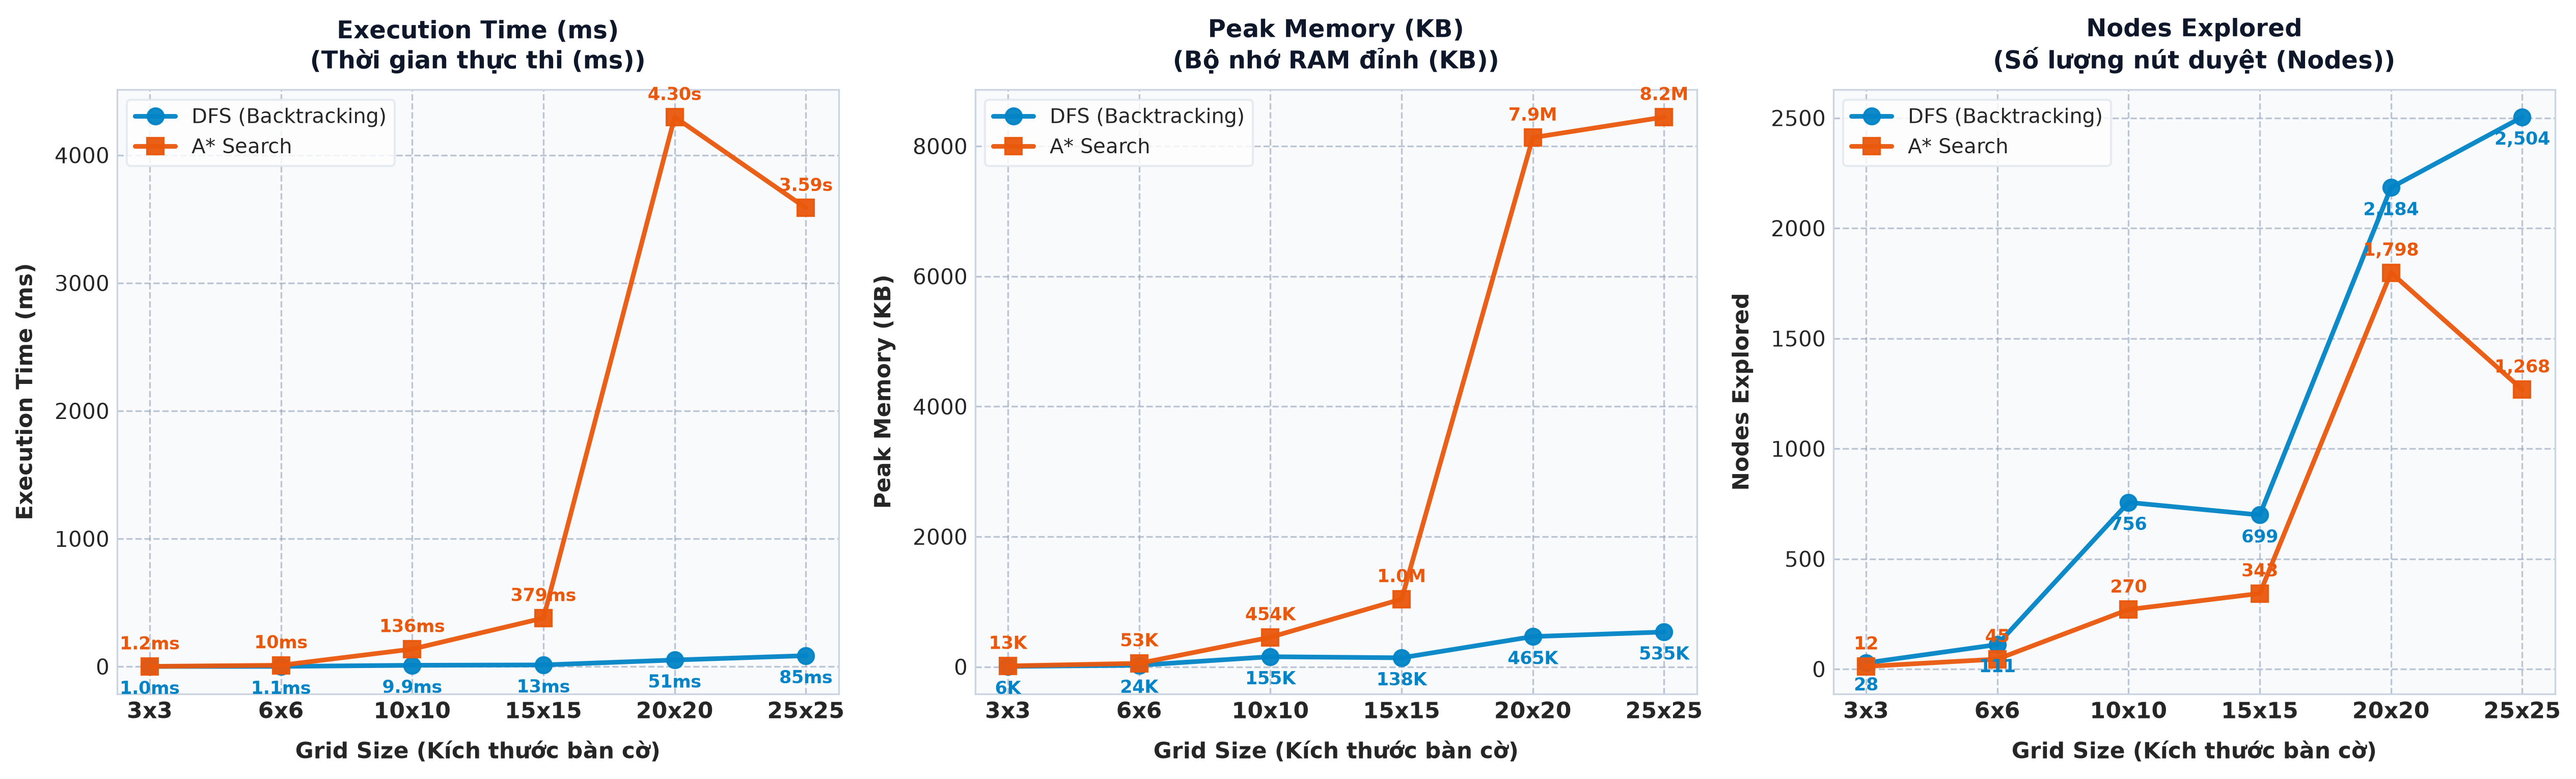
\includegraphics[width=1.0\textwidth]{Images/benchmark_summary.png}
\caption{Biểu đồ tổng hợp 3 thông số thực nghiệm: Thời gian thực thi (ms), Bộ nhớ RAM đỉnh (KB) và Số lượng nút duyệt (Nodes Explored) khi kích thước bàn cờ tăng đều đặn từ $3 \times 3$ đến $25 \times 25$ ($625$ ô).}
\label{fig:benchmark_summary}
\end{figure}

\begin{figure}[H]
\centering
\begin{subfigure}[b]{0.48\textwidth}
    \centering
    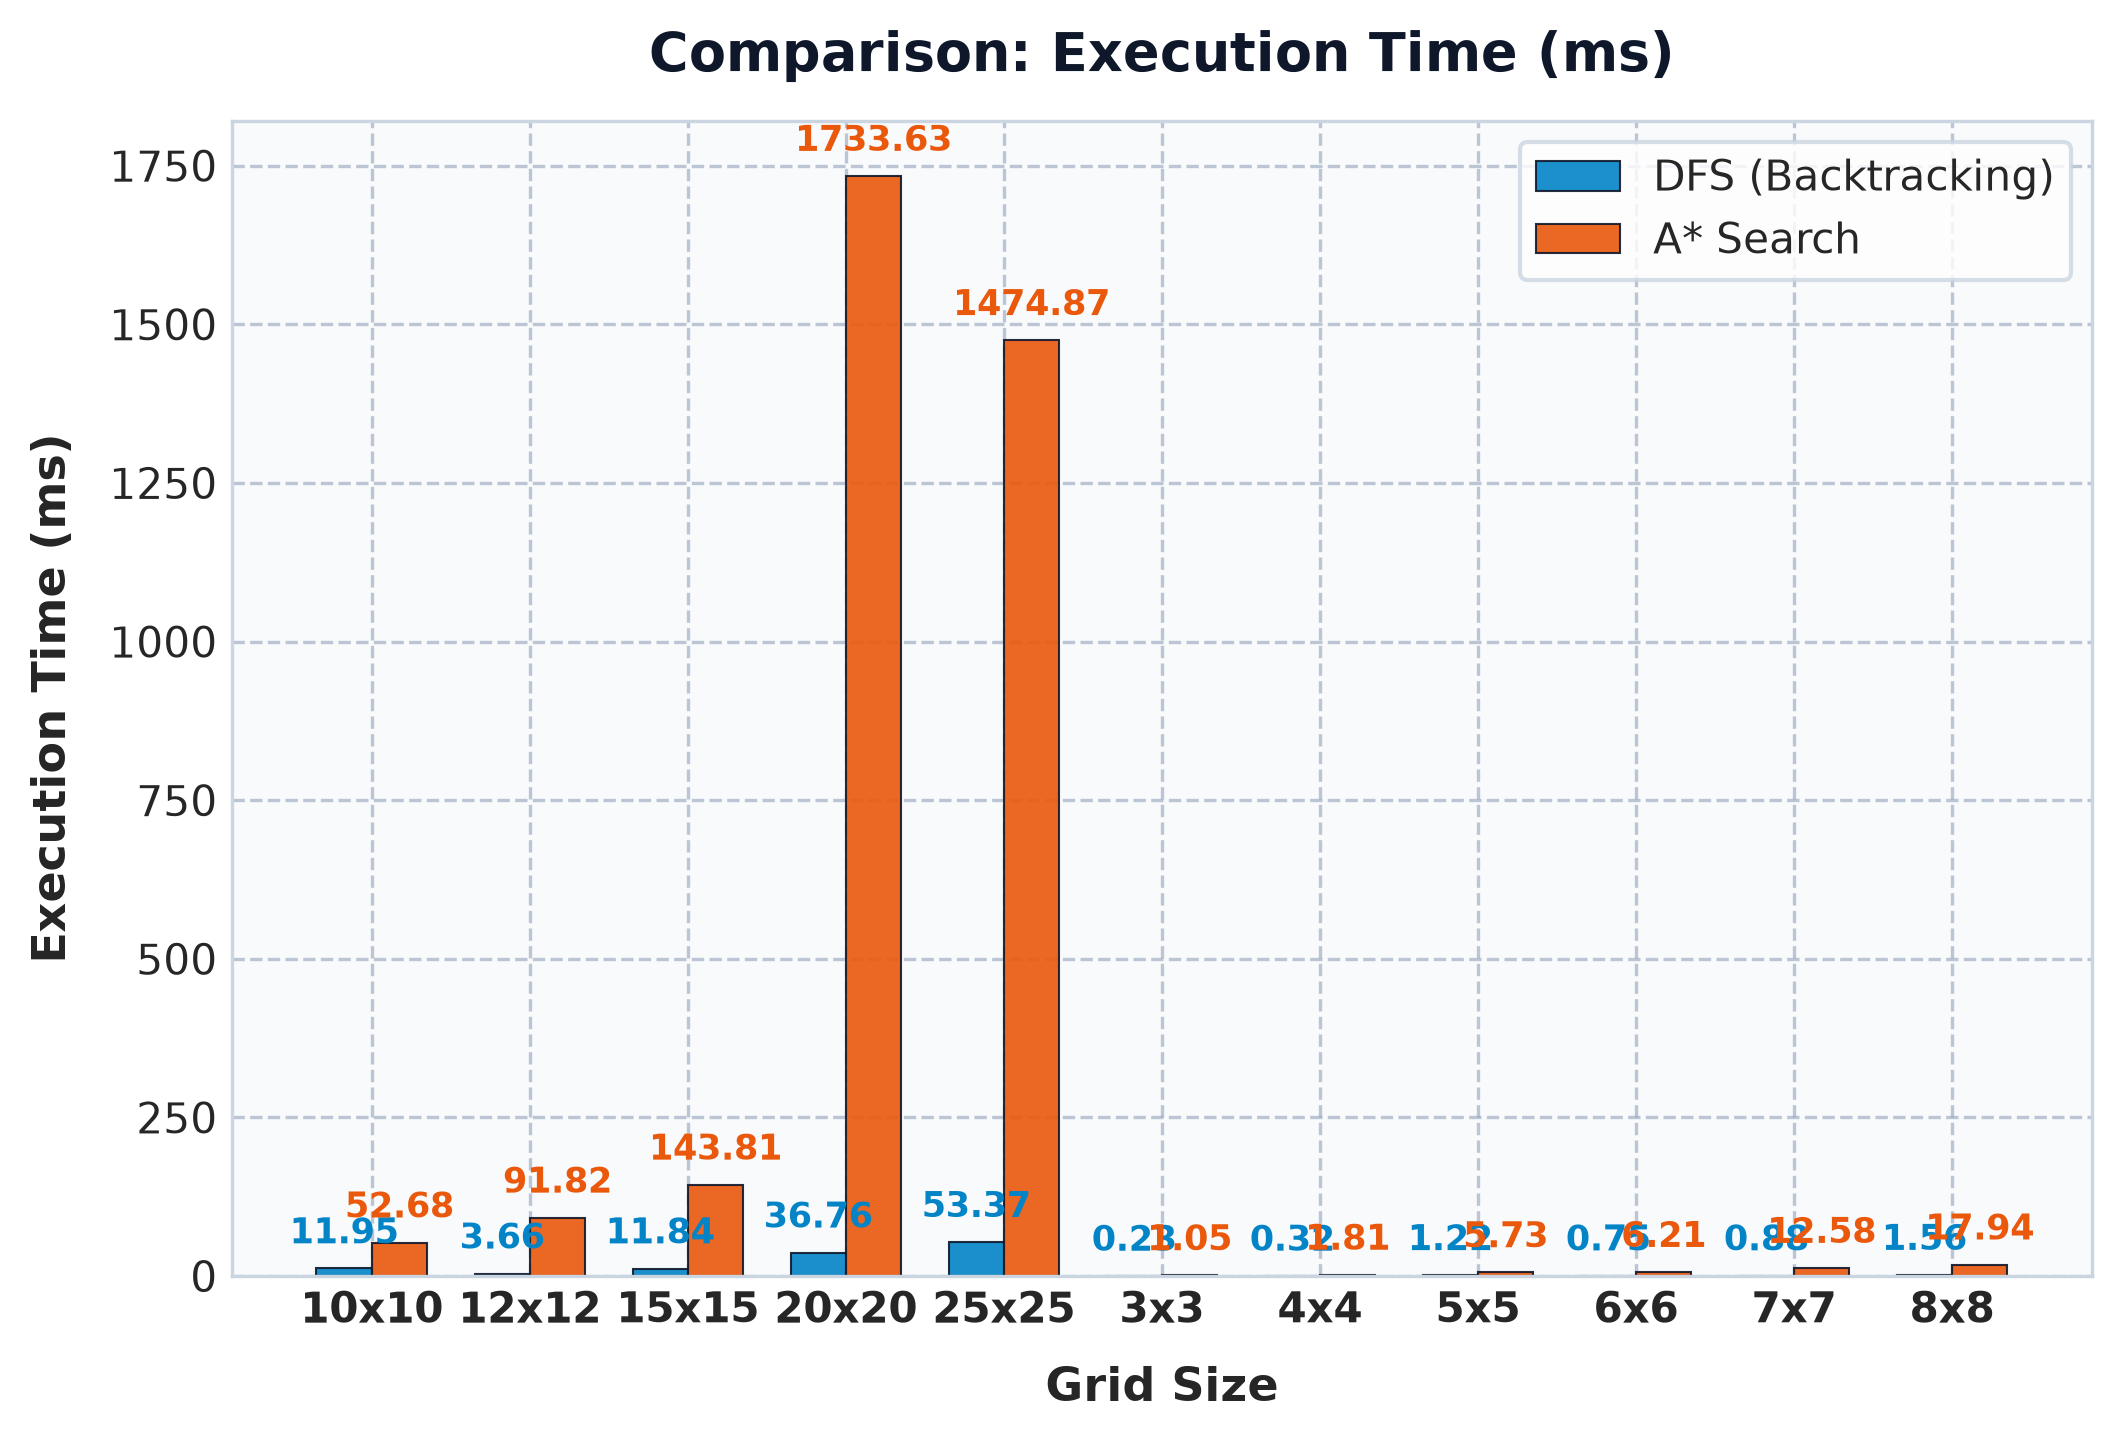
\includegraphics[width=\textwidth]{Images/chart_time.png}
    \caption{So sánh Thời gian thực thi (ms)}
    \label{fig:chart_time}
\end{subfigure}
\hfill
\begin{subfigure}[b]{0.48\textwidth}
    \centering
    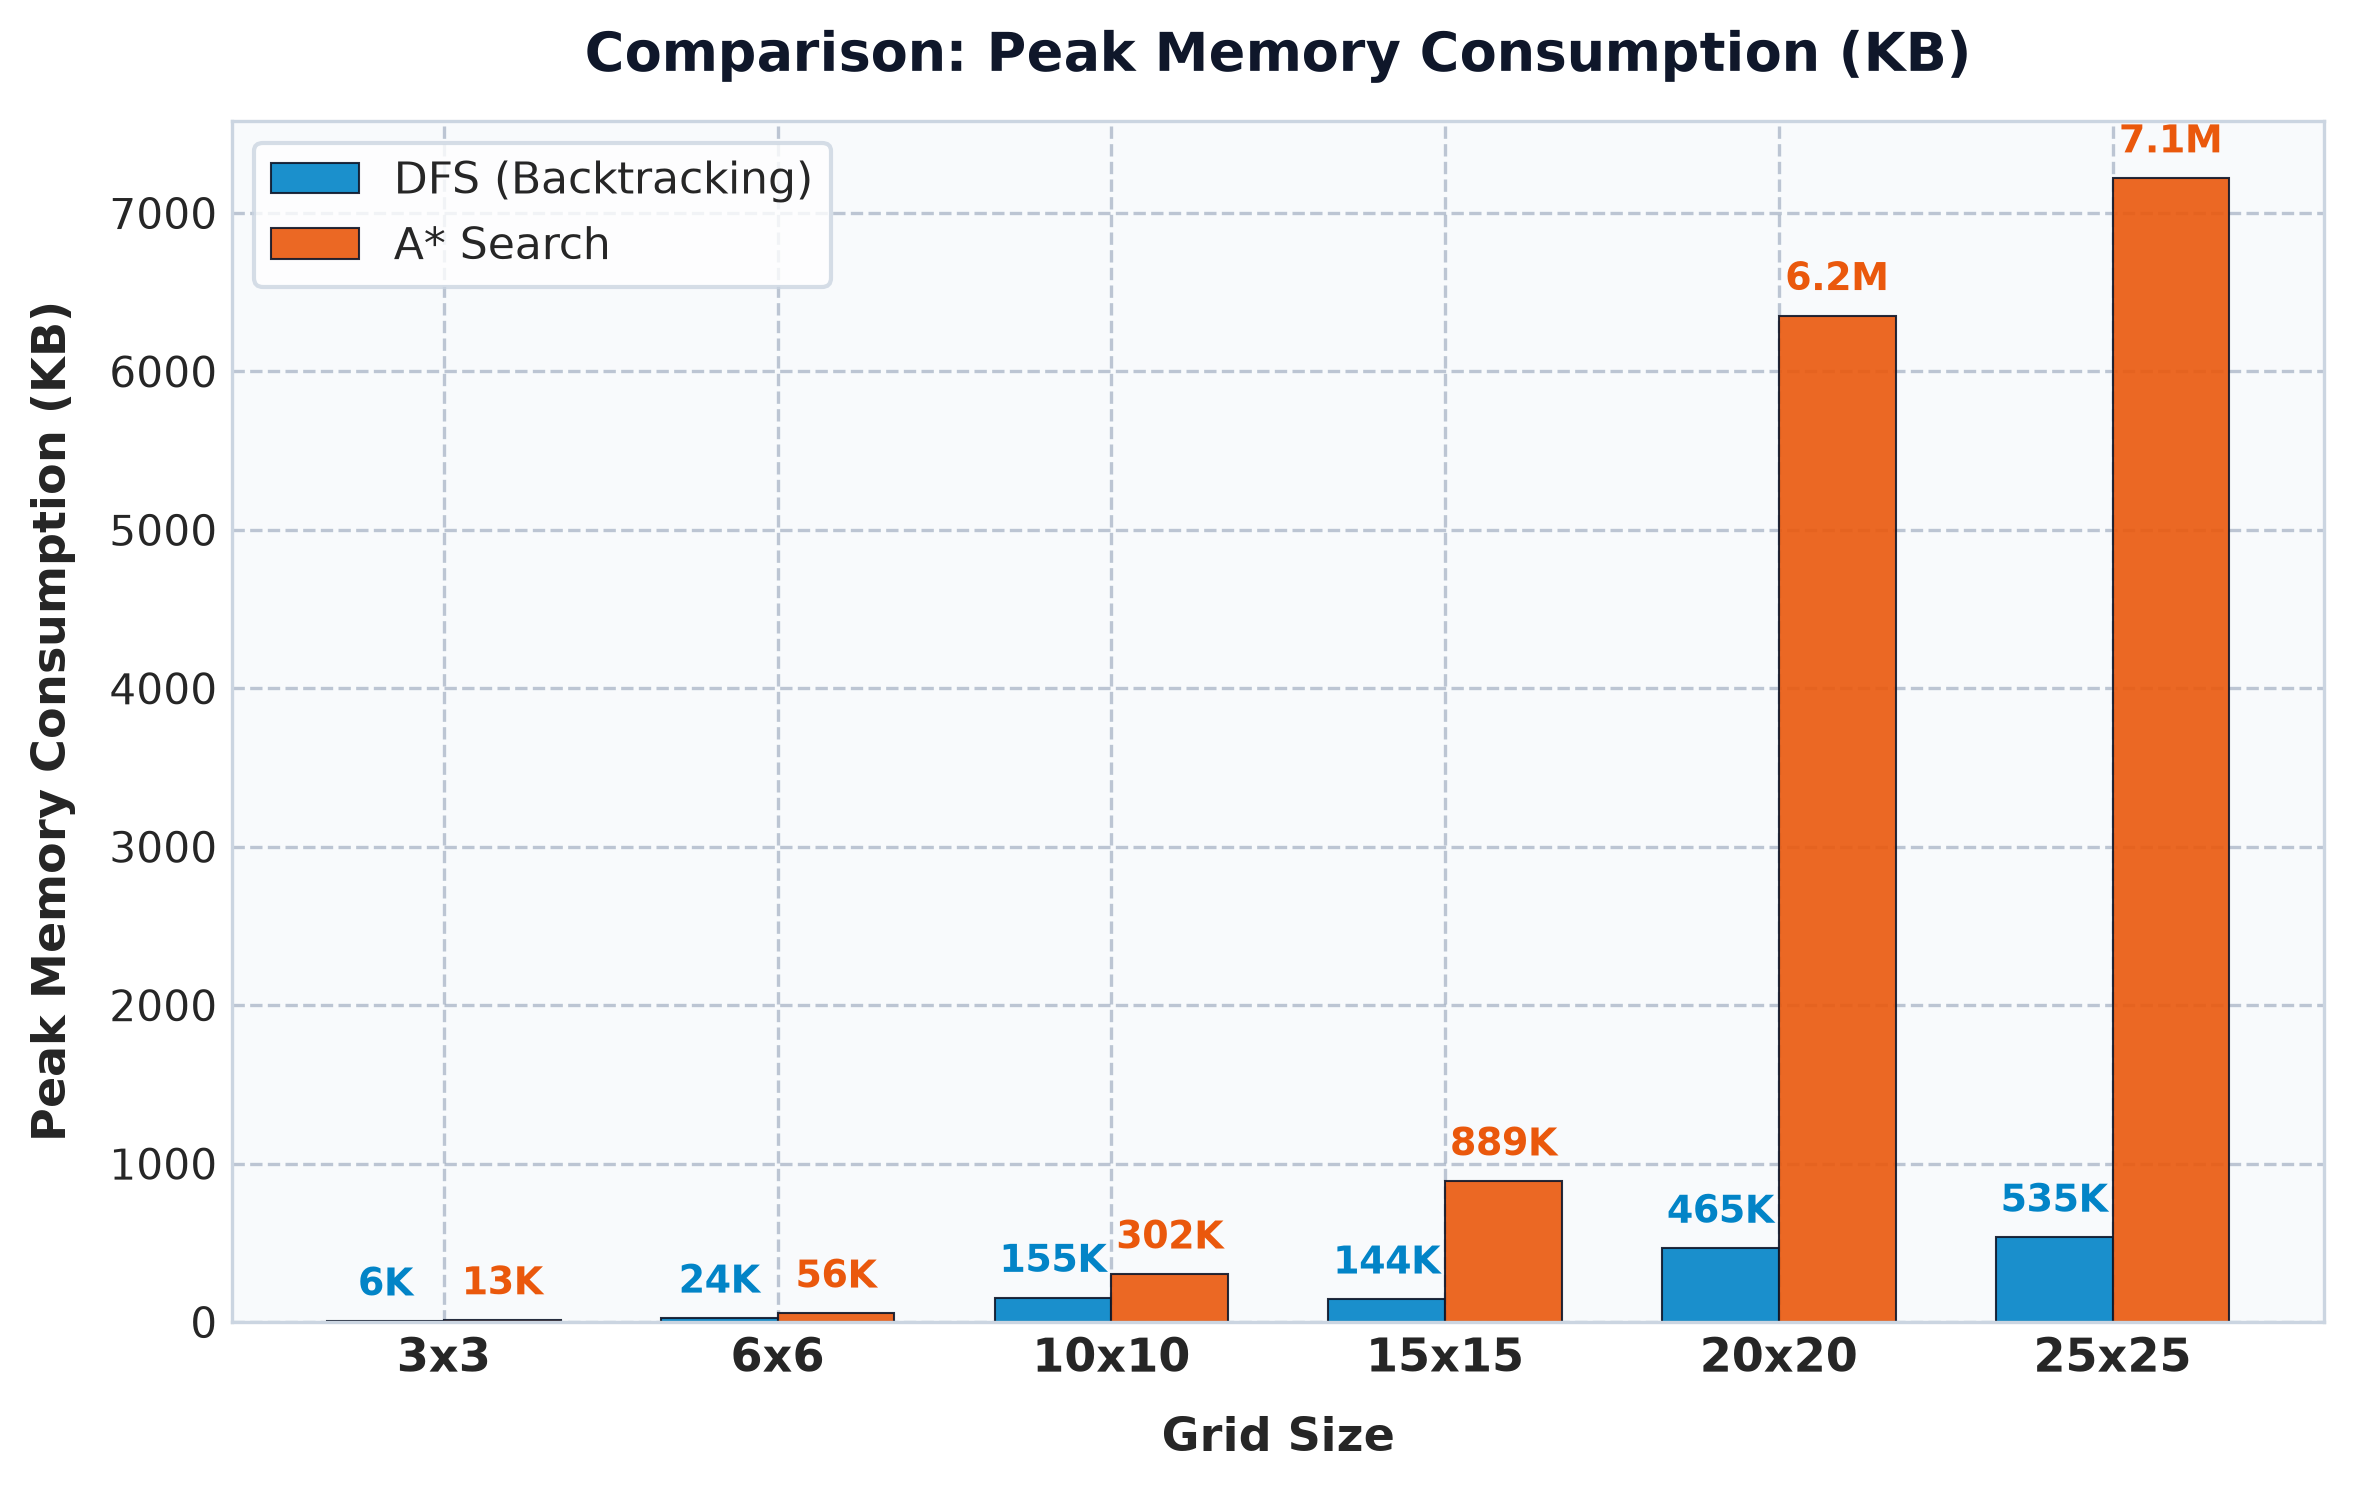
\includegraphics[width=\textwidth]{Images/chart_memory.png}
    \caption{So sánh Bộ nhớ tiêu thụ đỉnh (KB)}
    \label{fig:chart_memory}
\end{subfigure}

\vspace{0.3cm}
\begin{subfigure}[b]{0.52\textwidth}
    \centering
    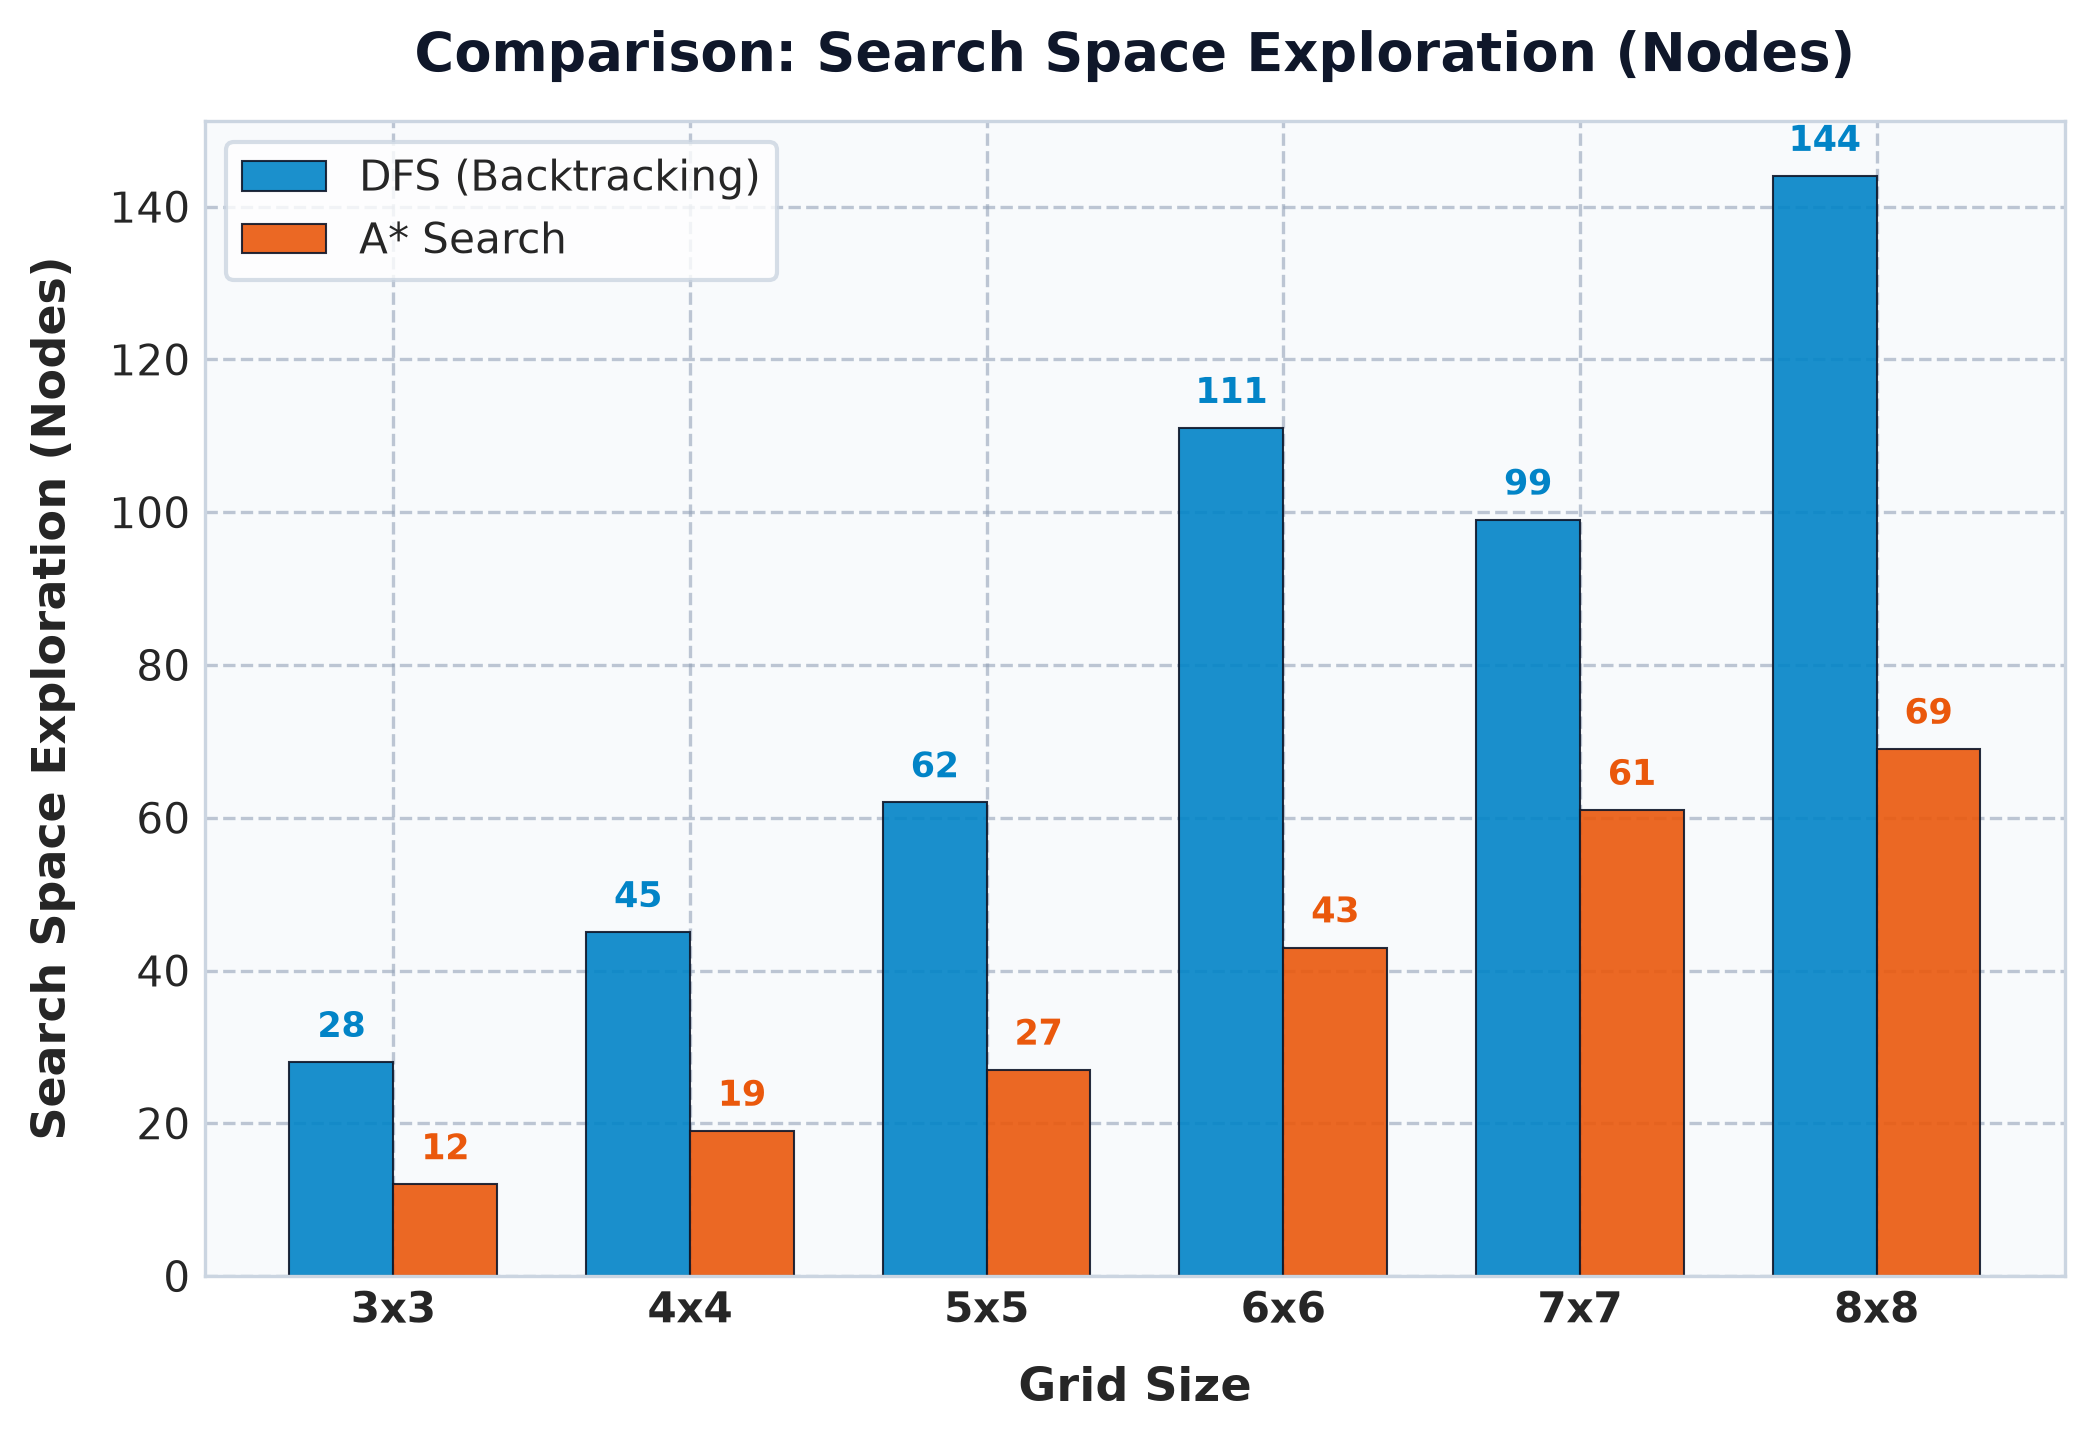
\includegraphics[width=\textwidth]{Images/chart_nodes.png}
    \caption{So sánh Số lượng nút trạng thái đã duyệt (Nodes)}
    \label{fig:chart_nodes}
\end{subfigure}
\caption{Biểu đồ cột chi tiết từng tiêu chí hiệu năng giữa DFS (Backtracking) và $A^*$ Search.}
\label{fig:individual_charts}
\end{figure}

\subsection{Phân tích và Giải thích kết quả thực nghiệm}
Quan sát Bảng \ref{tab:benchmark_results} và các đồ thị trong Hình \ref{fig:benchmark_summary}, \ref{fig:individual_charts}, kết quả thực nghiệm phản ánh một hiện tượng rất kinh điển trong lý thuyết Trí tuệ nhân tạo: \textbf{sự đánh đổi (trade-off) giữa tri thức Heuristic và chi phí quản lý trạng thái}.

\subsubsection{Giải thích về Số lượng nút đã duyệt (Nodes Explored)}
\begin{itemize}
    \item \textbf{Xu hướng thực nghiệm:} Trên toàn bộ 6 bộ kiểm thử từ $3 \times 3$ đến $25 \times 25$, thuật toán $A^*$ Search luôn mở rộng số nút trạng thái ít hơn vượt trội so với DFS (chỉ bằng khoảng $40\% - 60\%$ số nút của DFS). Đặc biệt ở bàn cờ cực đại $25 \times 25$ ($625$ ô), $A^*$ chỉ cần duyệt $1044$ nút, trong khi DFS phải duyệt tới $2504$ nút.
    \item \textbf{Nguyên nhân bản chất:} 
    DFS là giải thuật tìm kiếm mù, tại mỗi ô $(r, c)$ nó chỉ thử các cấu hình xoay theo thứ tự cố định. Khi chọn nhầm một góc xoay ở hàng trên nhưng cục bộ vẫn khớp, DFS phải đào sâu xuống nhiều tầng bên dưới trước khi nhận ra mâu thuẫn và buộc phải quay lui hàng loạt.
    Ngược lại, $A^*$ sử dụng hàm Heuristic $h(n) = \text{remaining} + \lfloor \text{conflicts}/2 \rfloor$ để lượng hóa mức độ bất tương thích toàn cục. Nhờ đó, $A^*$ luôn ưu tiên bốc từ Min-Heap các trạng thái có hàm đánh giá $f(n)$ nhỏ nhất, định hướng đường đi thẳng tới nghiệm mà hiếm khi bị sa lầy vào các nhánh ngõ cụt.
\end{itemize}

\subsubsection{Giải thích về Thời gian thực thi (Execution Time)}
\begin{itemize}
    \item \textbf{Xu hướng thực nghiệm:} Mặc dù duyệt nhiều nút hơn, DFS lại có tốc độ giải nhanh hơn $A^*$ đáng kể ở mọi cấp độ: từ $0.92\text{ ms}$ ($3 \times 3$) lên $84.25\text{ ms}$ ($25 \times 25$). Trong khi đó, $A^*$ mất từ $1.06\text{ ms}$ ($3 \times 3$) lên đến khoảng $2.43\text{ s}$ ($25 \times 25$).
    \item \textbf{Nguyên nhân bản chất:}
    \begin{itemize}
        \item \textbf{Chi phí trên mỗi nút của DFS là $O(1)$:} DFS tận dụng cơ chế thay đổi trạng thái tại chỗ (\textit{in-place mutation}) trên duy nhất một ma trận bitmask. Khi thử một góc xoay, phép gán bitmask và phép kiểm tra khớp 2 ô láng giềng kề cạnh đều diễn ra trong $O(1)$ chu kỳ CPU.
        \item \textbf{Chi phí trên mỗi nút của $A^*$ là $O(R \times C + \log |\text{OpenSet}|)$:} Với mỗi trạng thái được mở rộng, $A^*$ phải sao chép ma trận lưới để đưa vào tập mở, đồng thời quét lại toàn bộ bàn cờ để tính hàm $h(n)$. Khi bàn cờ đạt $25 \times 25 = 625$ ô, chi phí sao chép dữ liệu và quét ma trận trở nên rất tốn kém CPU, làm chậm tốc độ tổng thể dù số nút duyệt ít hơn.
    \end{itemize}
\end{itemize}

\subsubsection{Giải thích về Sự tiêu tốn bộ nhớ (Peak Memory Consumption)}
\begin{itemize}
    \item \textbf{Xu hướng thực nghiệm:} Mức tiêu thụ RAM đỉnh của DFS tăng rất chậm và tuyến tính theo độ sâu: từ $5.73\text{ KB}$ ($3 \times 3$) lên vỏn vẹn $534.54\text{ KB}$ ($25 \times 25$). Ngược lại, bộ nhớ của $A^*$ tăng rất mạnh: từ $13.11\text{ KB}$ ($3 \times 3$) lên tới $7220.73\text{ KB}$ ($\approx 7.22\text{ MB}$) ở bàn cờ $25 \times 25$ -- cao gấp $13.5$ lần so với DFS.
    \item \textbf{Nguyên nhân bản chất:}
    \begin{itemize}
        \item DFS chỉ lưu trữ ngăn xếp lời gọi đệ quy có chiều sâu tối đa bằng số ô của bàn cờ ($d = R \times C = 625$). Bộ nhớ chỉ là $O(R \times C)$, hoàn toàn không phụ thuộc vào hệ số phân nhánh.
        \item $A^*$ bắt buộc phải lưu toàn bộ biên tìm kiếm $\text{OpenSet}$ trong Min-Heap cùng tập các trạng thái đã ghé thăm $\text{Visited}$ để tránh lặp chu trình. Khi số lượng trạng thái chờ trong Heap lên đến hàng nghìn phần tử, mỗi phần tử đều giữ một bản sao lưới $625$ ô và mảng lịch sử, dẫn đến sự bùng nổ không gian lưu trữ theo cấp số nhân $O(b^d)$.
    \end{itemize}
\end{itemize}

\subsubsection{Bảng tổng kết đối sánh hai giải thuật}
\begin{table}[H]
\centering
\caption{Tổng hợp ưu nhược điểm và phạm vi áp dụng của DFS (Backtracking) và $A^*$ Search.}
\label{tab:algo_comparison}
\renewcommand{\arraystretch}{1.35}
\begin{tabularx}{\textwidth}{|>{\raggedright\arraybackslash}p{3.0cm}|>{\raggedright\arraybackslash}X|>{\raggedright\arraybackslash}X|}
\hline
\textbf{Tiêu chí so sánh} & \textbf{DFS (Backtracking + Pruning)} & \textbf{A* Search (Min-Heap)} \\
\hline
Bản chất tìm kiếm & Tìm kiếm mù kết hợp cắt tỉa ràng buộc cục bộ (Forward Pruning). & Tìm kiếm có thông tin định hướng bởi hàm đánh giá $f(n) = g(n) + h(n)$. \\
\hline
Số nút duyệt (Nodes) & Nhiều hơn (do thử-sai tuần tự và quay lui khi gặp ngõ cụt). & Ít hơn từ $40\% - 60\%$ (nhờ Heuristic dẫn đường chính xác). \\
\hline
Tốc độ thực thi & Cực nhanh ($< 85\text{ ms}$ trên mọi bàn cờ đến $25 \times 25$) nhờ sửa trạng thái tại chỗ $O(1)$. & Chậm hơn khi ma trận lớn ($\approx 2.4\text{ s}$ ở $25 \times 25$) do chi phí tính $h(n)$ và quản lý Heap. \\
\hline
Tiêu tốn bộ nhớ & Cực kỳ tối ưu ($O(R \times C)$), chỉ tốn $\approx 535\text{ KB}$ ở $25 \times 25$. & Tăng nhanh theo kích thước bàn cờ ($\approx 7.22\text{ MB}$ ở $25 \times 25$) do lưu trữ $\text{OpenSet}$. \\
\hline
Phạm vi phù hợp & Rất phù hợp cho các bài toán giải đố logic dạng ô lưới có ràng buộc chặt. & Phù hợp cho bài toán tìm đường đi ngắn nhất hoặc khi hàm Heuristic tính toán rất rẻ. \\
\hline
\end{tabularx}
\end{table}

\newpage

% =====================================================================
% PHẦN 5: KẾT LUẬN VÀ HƯỚNG PHÁT TRIỂN
% =====================================================================
\section{Kết luận và Hướng phát triển}

\subsection{Kết luận}
Qua quá trình nghiên cứu và thực hiện Bài tập lớn 1, nhóm đã hoàn thành xuất sắc các mục tiêu đề ra:
\begin{enumerate}
    \item \textbf{Về mô hình hóa bài toán:} Xây dựng thành công mô hình toán học cho trò chơi Logic Puzzle Pipes dựa trên hệ thống Bitmask 4-bit, chuyển hóa toàn bộ các phép kiểm tra khớp nối và xoay góc hình học thành các phép toán dịch bit cấp thấp siêu nhanh.
    \item \textbf{Về hiện thực giải thuật:} Hiện thực hoàn chỉnh bằng Python 3 hai giải thuật tìm kiếm đại diện cho hai trường phái: DFS Backtracking kết hợp Forward Pruning (Blind Search) và $A^*$ Search với hàng đợi ưu tiên Min-Heap (Heuristic Search). Cả hai giải thuật đều giải chính xác $100\%$ toàn bộ các bộ kiểm thử từ nhỏ ($3 \times 3$) đến quy mô cực đại ($25 \times 25$ -- 625 ô).
    \item \textbf{Về thực nghiệm và đánh giá:} Thiết lập hệ thống đo đạc khách quan bằng \texttt{time.perf\_counter} và \texttt{tracemalloc}. Kết quả thực nghiệm làm sáng tỏ nguyên lý cơ bản của Trí tuệ nhân tạo: $A^*$ tiết kiệm số lượng nút mở rộng nhờ tri thức Heuristic, nhưng đối với các bài toán thỏa mãn ràng buộc có cấu trúc lưới cố định như Puzzle Pipes, DFS kết hợp cắt tỉa sớm (Forward Pruning) và cập nhật tại chỗ lại chiếm ưu thế vượt trội về tốc độ CPU và tiết kiệm bộ nhớ RAM.
    \item \textbf{Về giao diện trực quan:} Xây dựng ứng dụng Web Visualizer hiện đại, thân thiện, hỗ trợ chạy từng bước (Step-by-step), tự động phát, chỉnh tốc độ, 2 chế độ sáng/tối và tính năng tự động co giãn lưới thông minh cho mọi kích thước màn chơi.
\end{enumerate}

\newpage
\begin{thebibliography}{80}
\addcontentsline{toc}{section}{Tài liệu tham khảo}

\bibitem{russell2020}
Stuart Russell and Peter Norvig, \textit{Artificial Intelligence: A Modern Approach}, 4th Edition, Pearson, 2020. (Chương 3: Solving Problems by Searching \& Chương 6: Constraint Satisfaction Problems).

\bibitem{pipes_web}
Puzzle Team, ``Puzzle Pipes -- Online Logic Puzzle Game,'' [Online]. Available: \url{https://www.puzzle-pipes.com/}. [Accessed: Oct. 2026].

\bibitem{python_docs}
Python Software Foundation, ``\texttt{heapq} --- Heap queue algorithm \& \texttt{tracemalloc} --- Trace memory allocations,'' Python 3.10+ Standard Library Documentation. [Online]. Available: \url{https://docs.python.org/3/library/}.

\bibitem{cs_bku}
Khoa Khoa học và Kỹ thuật Máy tính -- Trường Đại học Bách Khoa ĐHQG-HCM, Tài liệu bài giảng môn Nhập môn Trí tuệ nhân tạo (CO3061), Học kỳ 1 năm học 2026--2027.

\end{thebibliography}
\end{document}
